\documentclass[a4paper,12pt,twoside]{memoir}

% Castellano
\usepackage[spanish,es-tabla]{babel}
\selectlanguage{spanish}
\usepackage[utf8]{inputenc}
\usepackage[T1]{fontenc}
\usepackage{lmodern} % scalable font
\usepackage{microtype}
\usepackage{placeins}
\usepackage{adjustbox}
\usepackage{tabularx}
\usepackage{placeins}

% Moneda
\usepackage{eurosym}

\RequirePackage{booktabs}
\RequirePackage[table]{xcolor}
\RequirePackage{xtab}
\RequirePackage{multirow}

% SVG 
\usepackage{svg}

% Landscape
\usepackage{pdflscape}

% Multi-page tables using
\usepackage{longtable}

% Links
\PassOptionsToPackage{hyphens}{url}\usepackage[colorlinks]{hyperref}
\hypersetup{
	allcolors = {red}
}

% Ecuaciones
\usepackage{amsmath}

% Rutas de fichero / paquete
\newcommand{\ruta}[1]{{\sffamily #1}}

% Párrafos
\nonzeroparskip

% Huérfanas y viudas
\widowpenalty100000
\clubpenalty100000

% Evitar solapes en el header
\nouppercaseheads

% Code
\usepackage{listings}
\usepackage{color}

\definecolor{dkgreen}{rgb}{0,0.6,0}
\definecolor{gray}{rgb}{0.5,0.5,0.5}
\definecolor{mauve}{rgb}{0.58,0,0.82}
\lstset{frame=tb,
  aboveskip=3mm,
  belowskip=3mm,
  showstringspaces=false,
  columns=flexible,
  basicstyle={\small\ttfamily},
  numbers=none,
  numberstyle=\tiny\color{gray},
  keywordstyle=\color{blue},
  commentstyle=\color{red},
  stringstyle=\color{mauve},
  breaklines=true,
  breakatwhitespace=true,
  tabsize=3,
  captionpos=b
}


% Imagenes
\usepackage{graphicx}
\newcommand{\imagen}[2]{
	\begin{figure}[!h]
		\centering
		\includegraphics[width=0.9\textwidth]{#1}
		\caption{#2}\label{fig:#1}
	\end{figure}
	\FloatBarrier
}

\newcommand{\imagenRuta}[3]{
	\begin{figure}[!h]
		\centering
		\includegraphics[width=0.9\textwidth]{#1}
		\caption{#2}\label{fig:#3}
	\end{figure}
	\FloatBarrier
}

\newcommand{\imagenFlotante}[3]{
	\begin{figure}%[!h]
		\centering
		\includegraphics[width=0.9\textwidth]{#1}
		\caption{#2}\label{fig:#3}
	\end{figure}
}

\newcommand{\imagenAncho}[4]{
	\begin{figure}[H]
		\centering
		\includegraphics[width=#4\textwidth]{#1}
		\caption{#2}\label{fig:#3}
	\end{figure}
	\FloatBarrier
}


% El comando \figura nos permite insertar figuras comodamente, y utilizando
% siempre el mismo formato. Los parametros son:
% 1 -> Porcentaje del ancho de página que ocupará la figura (de 0 a 1)
% 2 --> Fichero de la imagen
% 3 --> Texto a pie de imagen
% 4 --> Etiqueta (label) para referencias
% 5 --> Opciones que queramos pasarle al \includegraphics
% 6 --> Opciones de posicionamiento a pasarle a \begin{figure}
\newcommand{\figuraConPosicion}[6]{%
  \setlength{\anchoFloat}{#1\textwidth}%
  \addtolength{\anchoFloat}{-4\fboxsep}%
  \setlength{\anchoFigura}{\anchoFloat}%
  \begin{figure}[#6]
    \begin{center}%
      \Ovalbox{%
        \begin{minipage}{\anchoFloat}%
          \begin{center}%
            \includegraphics[width=\anchoFigura,#5]{#2}%
            \caption{#3}%
            \label{#4}%
          \end{center}%
        \end{minipage}
      }%
    \end{center}%
  \end{figure}%
}

%
% Comando para incluir imágenes en formato apaisado (sin marco).
\newcommand{\figuraApaisadaSinMarco}[5]{%
  \begin{figure}%
    \begin{center}%
    \includegraphics[angle=90,height=#1\textheight,#5]{#2}%
    \caption{#3}%
    \label{#4}%
    \end{center}%
  \end{figure}%
}
% Para las tablas
\newcommand{\otoprule}{\midrule [\heavyrulewidth]}
%
% Nuevo comando para tablas pequeñas (menos de una página).
\newcommand{\tablaSmall}[5]{%
 \begin{table}
  \begin{center}
   \rowcolors {2}{gray!35}{}
   \begin{tabular}{#2}
    \toprule
    #4
    \otoprule
    #5
    \bottomrule
   \end{tabular}
   \caption{#1}
   \label{tabla:#3}
  \end{center}
 \end{table}
}

%
%Para el float H de tablaSmallSinColores
\usepackage{float}

%
% Nuevo comando para tablas pequeñas (menos de una página).
\newcommand{\tablaSmallSinColores}[5]{%
 \begin{table}[H]
  \begin{center}
   \begin{tabular}{#2}
    \toprule
    #4
    \otoprule
    #5
    \bottomrule
   \end{tabular}
   \caption{#1}
   \label{tabla:#3}
  \end{center}
 \end{table}
}

\newcommand{\tablaApaisadaSmall}[5]{%
\begin{landscape}
  \begin{table}
   \begin{center}
    \rowcolors {2}{gray!35}{}
    \begin{tabular}{#2}
     \toprule
     #4
     \otoprule
     #5
     \bottomrule
    \end{tabular}
    \caption{#1}
    \label{tabla:#3}
   \end{center}
  \end{table}
\end{landscape}
}

%
% Nuevo comando para tablas grandes con cabecera y filas alternas coloreadas en gris.
\newcommand{\tabla}[6]{%
  \begin{center}
    \tablefirsthead{
      \toprule
      #5
      \otoprule
    }
    \tablehead{
      \multicolumn{#3}{l}{\small\sl continúa desde la página anterior}\\
      \toprule
      #5
      \otoprule
    }
    \tabletail{
      \hline
      \multicolumn{#3}{r}{\small\sl continúa en la página siguiente}\\
    }
    \tablelasttail{
      \hline
    }
    \bottomcaption{#1}
    \rowcolors {2}{gray!35}{}
    \begin{xtabular}{#2}
      #6
      \bottomrule
    \end{xtabular}
    \label{tabla:#4}
  \end{center}
}

%
% Nuevo comando para tablas grandes con cabecera.
\newcommand{\tablaSinColores}[6]{%
  \begin{center}
    \tablefirsthead{
      \toprule
      #5
      \otoprule
    }
    \tablehead{
      \multicolumn{#3}{l}{\small\sl continúa desde la página anterior}\\
      \toprule
      #5
      \otoprule
    }
    \tabletail{
      \hline
      \multicolumn{#3}{r}{\small\sl continúa en la página siguiente}\\
    }
    \tablelasttail{
      \hline
    }
    \bottomcaption{#1}
    \begin{xtabular}{#2}
      #6
      \bottomrule
    \end{xtabular}
    \label{tabla:#4}
  \end{center}
}

%
% Nuevo comando para tablas grandes sin cabecera.
\newcommand{\tablaSinCabecera}[5]{%
  \begin{center}
    \tablefirsthead{
      \toprule
    }
    \tablehead{
      \multicolumn{#3}{l}{\small\sl continúa desde la página anterior}\\
      \hline
    }
    \tabletail{
      \hline
      \multicolumn{#3}{r}{\small\sl continúa en la página siguiente}\\
    }
    \tablelasttail{
      \hline
    }
    \bottomcaption{#1}
  \begin{xtabular}{#2}
    #5
   \bottomrule
  \end{xtabular}
  \label{tabla:#4}
  \end{center}
}



\definecolor{cgoLight}{HTML}{EEEEEE}
\definecolor{cgoExtralight}{HTML}{FFFFFF}

%
% Nuevo comando para tablas grandes sin cabecera.
\newcommand{\tablaSinCabeceraConBandas}[5]{%
  \begin{center}
    \tablefirsthead{
      \toprule
    }
    \tablehead{
      \multicolumn{#3}{l}{\small\sl continúa desde la página anterior}\\
      \hline
    }
    \tabletail{
      \hline
      \multicolumn{#3}{r}{\small\sl continúa en la página siguiente}\\
    }
    \tablelasttail{
      \hline
    }
    \bottomcaption{#1}
    \rowcolors[]{1}{cgoExtralight}{cgoLight}

  \begin{xtabular}{#2}
    #5
   \bottomrule
  \end{xtabular}
  \label{tabla:#4}
  \end{center}
}




\graphicspath{ {./img/} }

% Capítulos
\chapterstyle{bianchi}
\newcommand{\capitulo}[2]{
	\setcounter{chapter}{#1}
	\setcounter{section}{0}
	\setcounter{figure}{0}
	\setcounter{table}{0}
	\chapter*{#2}
	\addcontentsline{toc}{chapter}{#2}
	\markboth{#2}{#2}
}

% Apéndices
\renewcommand{\appendixname}{Apéndice}
\renewcommand*\cftappendixname{\appendixname}

\newcommand{\apendice}[1]{
	%\renewcommand{\thechapter}{A}
	\chapter{#1}
}

\renewcommand*\cftappendixname{\appendixname\ }

% Formato de portada
\makeatletter
\usepackage{xcolor}
\newcommand{\tutor}[1]{\def\@tutor{#1}}
\newcommand{\course}[1]{\def\@course{#1}}
\definecolor{cpardoBox}{HTML}{E6E6FF}
\def\maketitle{
  \null
  \thispagestyle{empty}
  % Cabecera ----------------
\noindent
\includegraphics[width=\textwidth]{cabecera}\vspace{1cm}%
  \vfill
  % Título proyecto y escudo informática ----------------
  \colorbox{cpardoBox}{%
    \begin{minipage}{.8\textwidth}
      \vspace{.5cm}\Large
      \begin{center}
      \textbf{TFG del Grado en Ingeniería Informática}\vspace{.6cm}\\
      \textbf{\LARGE\@title{}}
      \end{center}
      \vspace{.2cm}
    \end{minipage}

  }%
  \hfill\begin{minipage}{.20\textwidth}
    
\includegraphics[width=\textwidth]{escudoInfor}
  \end{minipage}
  \vfill
  % Datos de alumno, curso y tutores ------------------
  \begin{center}%
  {%
    \noindent\LARGE
    Presentado por \@author{}\\ 
    en Universidad de Burgos --- \@date{}\\
    Tutor: \@tutor{}\\
  }%
  \end{center}%
  \null
  \cleardoublepage
  }
\makeatother


% Datos de portada
\title{Estudio de métodos de selección de instancias en aprendizaje Semi-Supervisado y aplicación web de MLaaS\\Documentación Técnica}
\author{Daniel Puente Ramírez}
\tutor{Dr. Álvar Arnaiz González}
\date{\today}

\begin{document}

\maketitle



\cleardoublepage



%%%%%%%%%%%%%%%%%%%%%%%%%%%%%%%%%%%%%%%%%%%%%%%%%%%%%%%%%%%%%%%%%%%%%%%%%%%%%%%%%%%%%%%%



\frontmatter


\clearpage

% Indices
\tableofcontents

\clearpage

\listoffigures

\clearpage

\listoftables

\clearpage

\mainmatter

\appendix

\apendice{Plan de Proyecto Software}
\section{Introducción}
En este anexo se tratará el plan de proyecto, es la base sobre la que se crea el proyecto. Desde el punto de vista de la temporalidad y la viabilidad. Es una parte fundamental del ya que permitirá visualizar el escenario en el que se desarrollará el proyecto, permitiendo hacer una alineación estratégica de todos los elementos que se deben completar para finalizar correctamente el proyecto.

Desde el punto de vista de la planificación temporal, el proyecto sigue la metodología ágil \textit{Scrum}. Permitiendo definir cada uno de los objetivos que se desean alcanzar, los elementos que los componen y su respectiva prioridad.

\textit{Scrum}, de manera muy resumida, trabaja con u \textit{product backlog}, es una lista de prioridades en función del valor de cada tarea. Cuando comienza un \textit{sprint}, se empieza a trabajar en las tareas que se encuentren en el \textit{sprint backlog}, estas han sido extraídas del \textit{product backlog}. En el caso de este proyecto se realiza una reunión de planificación, \textit{sprint planning}, cada dos semanas aproximadamente.

Para el control y seguimiento se utiliza una herramienta externa, \textit{Zenhub}, la cual permite la definición de las tareas, el seguimiento de cada una de ellas en función de la planificación póker, seguimiento de cada \textit{sprint}, el versionado, etc.

Seguidamente se realizará un estudio de la viabilidad del proyecto, tanto a nivel económico como legal.
\newpage

\section{Planificación temporal}
\subsection{\textit{SCRUM}}
\textit{Scrum} es un marco de trabajo que permite el trabajo colaborativo en equipos. Permite que los equipos que trabajan en proyectos con esta metodología se organicen por sí mismos, siendo ellos los que deciden cómo afrontar los problemas que van surgiendo. 

Según \cite{cervone2011understanding}, el modelo \textit{Scrum} se basa en tres componentes principales: roles, procesos y artefactos. El \textit{Scrum Master} es el puesto asumido por el director o gerente del proyecto, o en algunos casos el líder del equipo. Esta figura representa los valores y principios por los que se rige la metodología de \textit{scrum}, manteniendo los valores y buenas prácticas, así como resolviendo los impedimentos que vayan surgiendo a lo largo del desarrollo del proyecto. Habitualmente los equipos están compuestos por entre cinco y diez personas que trabajan en el proyecto a tiempo completo. Siendo este equipo independiente y flexible en cuanto a jerarquía interna, no siendo representado el papel del ``jefe'' dentro de este por la misma persona siempre. Esto genera que el papel cambie en función de las necesidades del propio proyecto, la configuración del equipo cambia únicamente entre iteraciones, o \textit{sprints}, no dentro de los mismos.

\begin{figure}[]
	\centering
	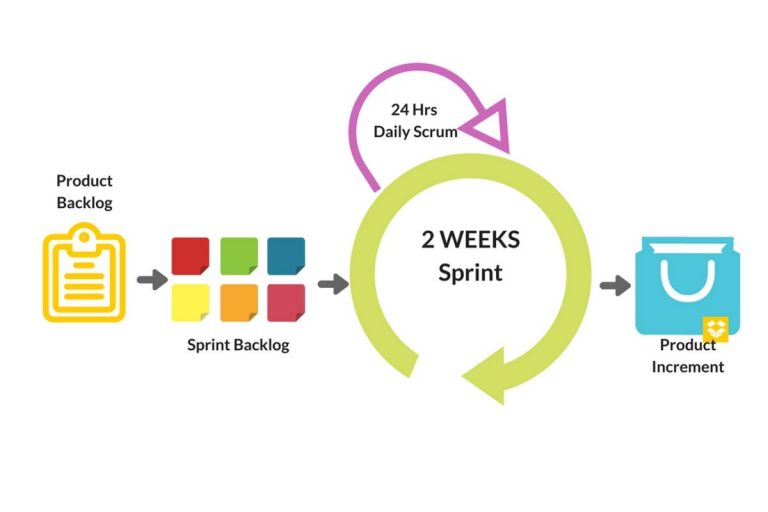
\includegraphics[scale=0.5]{../img/anexos/overview-scrum}
	\caption{Metodología \textit{scrum}.}\label{img:scrum-overview}
\end{figure}

\subsubsection{\textit{Sprints}}
Los \textit{sprints} son periodos breves de \textbf{tiempo fijo} en el que el equipo trabaja para completar una cantidad de trabajo pre-establecida. Si bien muchas guías asocian los \textit{sprints} a la metodología ágil, asociando la metodología ágil y la metodología seguida en \textit{scrum} como si fueran lo mismo, cuando no lo son. La metodología ágil constituye una serie de principios, y la metodología \textit{scrum} es un marco de trabajo con la única finalidad de conseguir resultados.

A pesar de las similitudes los \textit{sprints} poseen un objetivo subyacente, entregar con frecuencia \textit{software} de trabajo.

\subsubsection{\textit{Sprint meetings}}
Dentro de la metodología \textit{scrum} existen diferentes reuniones que favorecen la agilidad del proyecto y que todo el mundo sepa lo que tiene que hacer en cada momento.
\begin{itemize}
\item \textbf{\textit{Sprint planning meeting.}} Esta reunión puede tener una duración de hasta de un día completo de trabajo. En ella deben de estar presentes todas las partes del proyecto, i.e. el \textit{Scrum Master}, el equipo de desarrollo, y el \textit{product owner}. Poseen dos partes, en la primera de ellas se define el \textit{product backlog}, requerimientos del proyecto y se definen los objetivos para el \textit{sprint} que comienza, i.e. lo que se espera ``construir'' o completar en el \textit{sprint}. En la segunda parte de la reunión se trabaja en el \textit{sprint backlog}, las tareas que se van a seguir en el \textit{sprint} para completar el objetivo de éste.
\item \textbf{\textit{Daily meeting.}} Debido a que los requerimientos del proyecto no se pueden variar durante la vida de un \textit{sprint}, existen las reuniones diarias que son organizadas por el \textit{Scrum Master} en las que se comenta el trabajo del día previo, lo que se espera de ese día y qué está retrasando o impidiendo a un individuo el proseguir con sus tareas, esta reunión no debe tener una duración de más de quince minutos y se debe realizar ``de pie''. No es una reunión para ver quién retrasa el proyecto sino para ayudar a quién lo necesite entre todos los miembros del equipo y permitir esa agilidad.
\item \textbf{\textit{Sprint review meeting.}} Reunión fijada al final de cada \textit{sprint} en la cual se hace una puesta en conocimiento de lo que se ha realizado en ese \textit{sprint}, siempre que se pueda se hará una demostración funcional en lugar de una presentación al \textit{product owner}. Esta reunión tiene un carácter informal.
\end{itemize}
 
\subsubsection{Artifacts}
Uno de los componentes más importantes de cara a la metodología \textit{scrum} son los artefactos, o \textit{artifacts} por su nombre en inglés. Éstos incluyen el \textit{product backlog}, el \textit{sprint backlog} y los \textit{burn down charts}.
\begin{itemize}
\item \textbf{\textit{Product backlog.}} Lista de trabajo ordenada por las prioridades para el equipo de desarrollo. Es generada a partir de las reuniones de planificación de los \textit{sprints}, contiene los requisitos. Se encuentra actualizado y clasificado en función de la periodicidad asignada a las tareas, pudiendo ser de corto o largo plazo. Aquellas tareas que se deban resolver a corto plazo deberán estar perfectaemnte descritas antes de asignarlas esta periodicidad, implicnddo que se han diseñado las historias de usuario completas así como el equipo de desarrollo ha establecido las estimaciones correspondientes. Los elementos a largo plazo pueden ser abstractos u opacos, conviene que estén estimados en la medida de lo posible para poder tener en cuenta el tiempo que llevará desarrollarla.

Los propietarios del producto dictan la prioridad de los elementos de trabajo en el \textit{product backlog}, mientras que el equipo de desarrollo dicta la velocidad a la que se trabaja en \textit{backlog}.\cite{danradigan2021}

La estimación es una parte muy importante ya que es lo que permitirá al equipo de desarrollo mantener el ánimo y el trabajo al ritmo deseado. La estimación es realizada en la \textit{sprint planning meeting}, en la que se estima para cada tarea/producto del \textit{product backlog}. No se busca tener un resultado exacto del tiempo que va a llevar al equipo completar esa tarea, sino es una previsión. Para realizar correctamente la estimación se debe tener en cuenta el tamaño y la categoría de la tarea, los puntos de historia que se le van a asignar, así como el número de horas y días que van a ser necesarias para completar la tarea. 

\item \textbf{\textit{Sprint backlog.}} Lista de tareas extraídas del \textit{product backlog} que se han acordado desarrollarse a lo largo de un \textit{sprint}. Este \textit{backlog} es seleccionado por el propio equipo de desarrollo, para ello seleccionan una tarea del \textit{product backlog} y se divide en tareas de menor tamaño y abordables. Aquellas tareas de menor tamaño que el equipo no haya sido capaz de desarrollar previo a la finalización del \textit{sprint} quedarán almacenadas para próximos \textit{sprints} en el \textit{sprint backlog}.
\end{itemize}

\subsubsection{Actores, roles y responsabilidades}
Dentro de un equipo que sigue la metodología \textit{scrum} encontramos diferentes actores, como ya se ha comentado el equipo de desarrollo suele estar compuesto por entre cinco y diez personas, además del \textit{Scrum Master} y el \textit{Product Owner}.\cite{julioroche_2020}
\begin{itemize}
\item \textbf{\textit{Product Owner.}} Encargado de optimizar y maximizar el valor del producto, es la persona encargada de gestionar las prioridades del \textit{product backlog}. Una de sus principales tareas es la de intermediario con los \textit{stakeholders}, partes interesadas, del proyecto; junto con recoger los requerimientos de los clientes. Es habitual que esta figura sea representante del negocio, con lo que aumenta su valor.

Para cada \textit{sprint} debe de marcar el objetivo de éste de manera clara y acordada con el equipo de desarrollo, lo cual hará que el producto vaya incrementando constantemente su valor. Para que todo fluya como debe, esta figura tiene que tener el ``poder'' de tomar decisiones que afecten al producto.

\item \textbf{\textit{Scrum Master.}} Figura con dos responsabilidades, gestionar el proceso \textit{scrum} y ayudar a eliminar impedimentos que puedan afectar a la entrega del producto.
\begin{enumerate}
\item Gestionar el proceso \textit{scrum}. Su función es asegurarse de que el proceso se lleva a cabo correctamente, facilitando la ejecución de éste y sus mecánicas. Consiguiendo que la metodología sea una fuente de generación de valor.
\item Eliminar impedimentos. Eliminar los problemas que vayan surgiendo a lo largo de los \textit{sprints} con el fin de mantener el ritmo de trabajo dentro de los equipos de desarrollo para poder entregar valor, manteniendo la integridad de la metodología.
\end{enumerate}
\item \textbf{Equipo de desarrollo.} Formado por entre cinco y diez personas encargados del desarrollo del producto, organizados de forma autónoma para conseguir entregar las tareas del \textit{product backlog} asignadas al \textit{sprint} correspondiente. Para que funcione correctamente la metodología todos los integrantes deben de conocer su rol dentro del equipo, internamente se pueden gestionar como el equipo considere, pero de cara ``hacia fuera'' son un equipo con una responsabilidad.
\end{itemize}
\newpage
\subsection{Planificación por \textit{sprints}}
La organización temporal del proyecto se ha organizado siguiendo los estándares de la metodología \textit{scrum}, i.e. usando \textit{sprints}. 

Inicialmente la \textit{sprint planning meeting} es realizada cada dos semanas, debido a una falta de costumbre de trabajo con esta metodología se combina junto con la \textit{sprint review meeting}, de forma que en una sola reunión se comenta tanto lo que se ha hecho como lo que está por realizarse en el siguiente \textit{sprint}.

La velocidad de desarrollo del proyecto es una incógnita, debido a la no existencia de referencias previas del equipo de desarrollo del proyecto, en proyectos de ésta índole. Por lo tanto, la duración de los \textit{sprints} puede que se vea ajustada a lo largo de la vida del proyecto.

No se utilizan \textit{daily meetings} puesto que a pesar de que se invierte una media de tres a cinco horas diarias en el desarrollo, no es considerada necesaria. Si bien en caso de problemas se acuerda una reunión para el día siguiente con el fin de mantener la agilidad y no retrasar el proyecto.

\subsubsection{\textit{Sprint} 0: \textit{Lights out and away we go!} }
El \textit{sprint} con el que comienza el desarrollo de este proyecto no ha seguido la metodología \textit{scrum}, puesto que se formuló desde un punto de vista de toma de contacto inicial con el trabajo de investigación y todo lo que ello conlleva.

Los objetivos definidos han sido:
\begin{enumerate}
\item Lectura de \textit{papers} relacionados con el ámbito de la inteligencia artificial. En concreto \textit{SSL density peaks}\cite{wu2018self}, \textit{Co-Training}\cite{blum1998combining}, \textit{Tri-Training}\cite{zhou2005tri} y \textit{Democratic Co-Learning}\cite{zhou2004democratic}.
\end{enumerate}

El tiempo empleado en la lectura y asimilación de estos conceptos ha sido de catorce horas, es la primera vez que se leen \textit{papers} o artículos científicos completos procurando asimilar todos los conceptos de éstos. Se ha desarrollado entre el veintisiete de octubre y el cinco de noviembre, de dos mil veintiuno. 

\subsubsection{\textit{Sprint} 1: Chad}
\begin{itemize}
\item \textbf{\textit{Planning meeting}}

Objetivos del primer \textit{sprint}:
\begin{enumerate}
\item Lectura del API de \textit{scikit-learn}. Comprensión del funcionamiento de los transformadores y estimadores enfocado desde el punto de su programación.
\item Lectura de los \textit{papers On issues instance selection}\cite{liu2002issues}, \textit{Comparison of instances seletion algorithms I. algorithms survey}\cite{jankowski2004comparison} y \textit{Comparison of instance selection algorithms II. Results and comments}\cite{grochowski2004comparison}.
\item Implementación de las técnicas de reducción del conjunto de entrenamiento, basados en k-NN.
\end{enumerate}

\item \textbf{Marcas temporales}
El \textit{sprint} se desarrolla entre el ocho y el diecinueve de noviembre de dos mil veintiuno. Han sido dedicadas al desarrollo del proyecto treinta horas.

\item \textbf{\textit{Burndown chart}}
\begin{figure}
\begin{center}
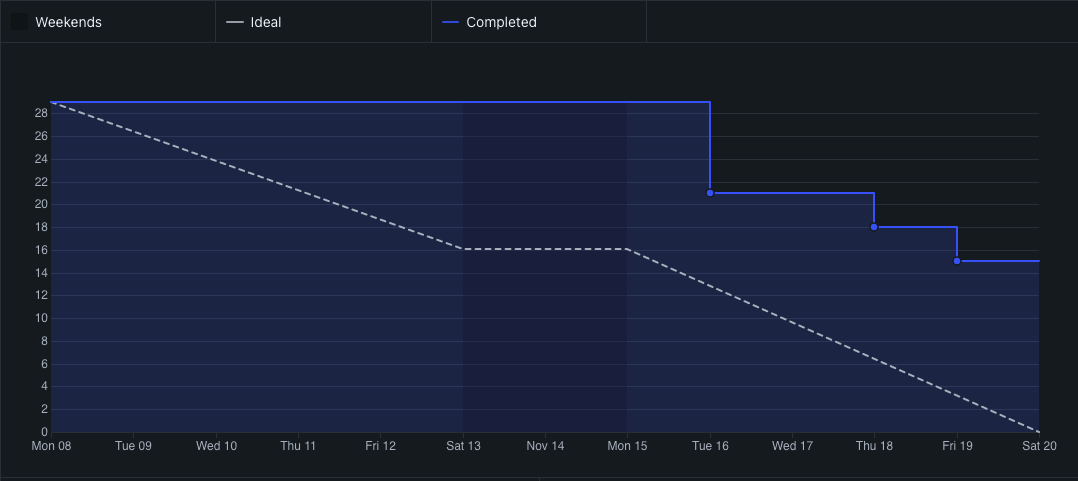
\includegraphics[width=\textwidth]{../img/anexos/sprints/BD-Sprint1}
\caption{\textit{Burndown Chart Sprint 1.}}\label{fig:BD-Sprint1}
\end{center}
\end{figure}
Durante este \textit{sprint} el trabajo inicial comenzó ligeramente retrasado, motivos en el apartado \textit{sprint review meeting}, por lo tanto podemos observar en la Figura \ref{fig:BD-Sprint1} como el trabajo completado dista del ideal o proyectado para este \textit{sprint}.

En el \textit{sprint backlog} habían sido incluidos todos los algoritmos a programar, es por ello que indica que se ha completado aproximadamente la mitad del trabajo.

\item \textbf{\textit{Sprint review meeting}}
El trabajo en este primer \textit{sprint} ha salido adelante correctamente. Al ser el primer \textit{sprint} ha habido un pequeño error de configuración del repositorio junto con la herramienta ZenHub, de ahí que en el \textit{burndown chart} de esta semana, Figura \ref{fig:BD-Sprint1}, aparezca como que la primera semana del \textit{sprint} no ha habido trabajo completado.

La adaptación a la metodología ágil ha resultado un poco compleja.
\end{itemize}

\subsubsection{\textit{Sprint} 2: Holleyman}
\begin{itemize}
\item \textbf{\textit{Planning meeting}}

Objetivos del segundo \textit{sprint}:
\begin{enumerate}
\item Finalizar implementación de los algoritmos basados en técnicas de reducción del conjunto de entrenamiento.
\item Añadir la documentación correspondiente a los algoritmos implementados.
\item Comprobar el rendimiento de los algoritmos implementados respecto a los resultados de una ejecución similar con el software \textit{Weka}.
\end{enumerate}
El \textit{sprint} se desarrolla entre el veintidós de noviembre y el tres de diciembre de dos mil veintiuno. Han sido dedicadas al desarrollo del proyecto treinta y ocho horas.

\item \textbf{\textit{Burndown chart}}
\begin{figure}
\begin{center}
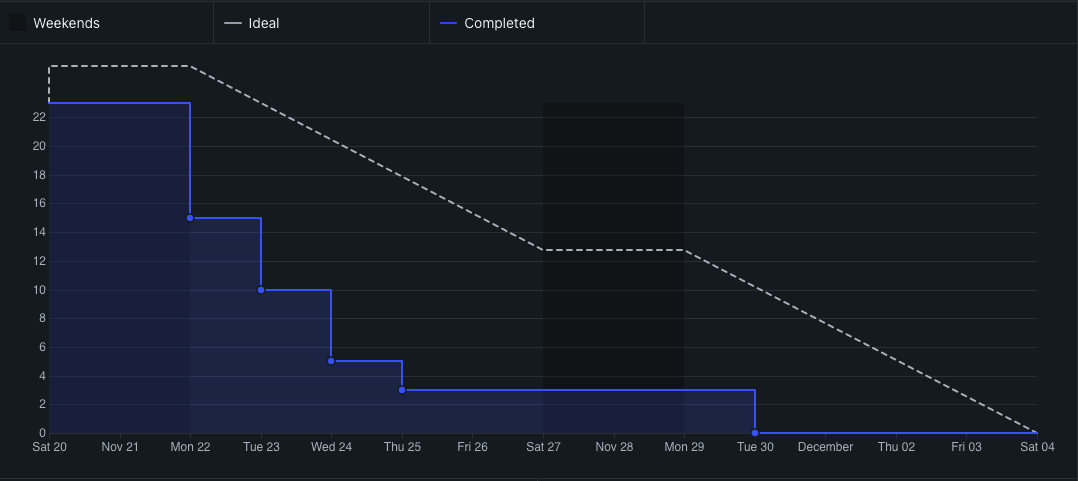
\includegraphics[width=\textwidth]{../img/anexos/sprints/BD-Sprint2}
\caption{\textit{Burndown Chart Sprint 2.}}\label{fig:BD-Sprint2}
\end{center}
\end{figure}

El trabajo realizado a lo largo de este \textit{sprint} ya ha sido adecuado a la metodología \textit{scrum}, obteniendo un \textit{burndown chart}, Figura \ref{fig:BD-Sprint2}, con más sentido que la que se había obtenido en el \textit{Sprint } 1. 

El equipo de desarrollo se sigue habituando poco a poco a la metodología de trabajo y en este \textit{sprint} se ha trabajo por debajo del ``ideal'' para el proyecto. 

\item \textbf{\textit{Sprint review meeting}}

A lo largo de este \textit{sprint} se descubrió un problema en la forma de identificar los k-NN en el algoritmo \textit{Condensed Nearest Neighbor, CNN}\cite{hart1968condensed}, retrasando el trabajo cuatro horas, entre identificación y re-programación. Este error se descubrió mientras se investigaba otro error, en este caso el algoritmo \textit{Iterative Case Filtering, ICF}\cite{brighton2002advances} terminaba en error buscando los k-NN de las últimas instancias.

La implementación de los algoritmos \textit{Reduced Nearest Neighbor, RNN}\cite{gates1972reduced} y \textit{Modified Selective Subset, MSS}\cite{barandela2005decision} ha sido relativamente asequible una vez se comprendía el algoritmo en cuestión así como su funcionamiento (entradas, procesado, salidas...).
\end{itemize}

\subsubsection{\textit{Sprint} 3: Manion}
\begin{itemize}
\item \textbf{\textit{Planning meeting}}

Objetivos del tercer \textit{sprint}:
\begin{enumerate}
\item Comenzar la documentación del proyecto.
\begin{itemize}
\item Comenzar la memoria por el marco teórico.
\item Comenzar los anexos por la planificación temporal.
\end{itemize} 
Se va a realizar en \LaTeX.
\item Aprender lo básico de \LaTeX lo más rápido posible para poder trabajar con él.
\item Buscar la precisión de los algoritmos implementados con conjuntos etiquetados de $[1\%, 5\%, 10\%, 20\%, 50\%]$ del conjunto total. En búsqueda de las asíntotas donde ya no mejora la clasificación.
\end{enumerate}
\item \textbf{Marcas temporales}

El \textit{sprint} se desarrolla entre el seis y el diecisiete de diciembre de dos mil veintiuno. Han sido dedicadas al desarrollo del proyecto XYZ horas.

\item \textbf{\textit{Burndown chart}}

\item \textbf{\textit{Sprint review meeting}}

\end{itemize}

\newpage
\subsubsection{\textit{Sprint} n: Name}
\begin{itemize}
\item \textbf{\textit{Planning meeting}}
\begin{enumerate}
\item Primero
\item Segundo
\end{enumerate}
\item \textbf{Marcas temporales}

\item \textbf{\textit{Burndown chart}}

\item \textbf{\textit{Sprint review meeting}}

\end{itemize}

\newpage
\section{Estudio de viabilidad}

\newpage
\subsection{Viabilidad económica}

\newpage
\subsection{Viabilidad legal}

\newpage












































































\apendice{Especificación de Requisitos}

\section{Introducción}
Este anexo recoge las necesidades funcionales que deberán ser soportadas por el sistema que va a ser desarrollado. Con el fin de obtener una buena documentación se deben identificar y describir los requisitos que debe el sistema satisfacer, pero sin entrar en cómo los va a resolver.

A día de hoy, no existe una autoridad que indique cómo se deben de realizar las especificaciones de requisitos \textit{software}, SRS. La comunidad se encuentra dividida entre <<la vieja escuela>> siguiendo guías de buenas prácticas (IEEE 830-1998~\cite{720574} ó 12207-2-2020~\cite{IEEE1220722020}), en contraposición con el \textit{Agile Manifiesto}, donde no se hace una especificación formal de toda la aplicación sino que cada 2-4 semanas se revisa y <<rehace>> en función de las necesidades del cliente.

Se va a realizar una combinación de ambos, por un lado se trabaja a lo largo del proyecto con una planificación ágil, y por otro se va a tener como referencia una especificación de requisitos que va a seguir la guía de buenas prácticas IEEE 830-1998. Ésta última recoge los siguientes puntos como referencias a una buena especificación de requisitos \textit{software}~\cite{ingenieriasoftwareytiemporeal_2020}.
\begin{itemize}
\item \textbf{Correcto.} Será correcto si, y sólo si, cada requisito declarado se encuentra en el \textit{software} entregado.
\item \textbf{Inequívoco.} Será inequívoco si, y solo si, cada requisitos declarado tiene sólo una interpretación. Cada característica de la última versión del producto se deberá describir con un único término.
\item \textbf{Completo.} Será completo si, y sólo si, incluye:
\begin{enumerate}
\item Los requisitos están relacionados a la funcionalidad, el desarrollo, las restricciones del diseño, los atributos y las interfaces externas. En particular debe reconocerse cualquier requisito externo impuesta por una especificación del sistema y debe tratarse.
\item La definición de las respuestas del \textit{software} a todos los posibles datos de la entrada del sistema y a toda clase de situaciones.
\item Tener todas las etiquetas llenas y referencias a todas las figuras, tablas, diagramas en el SRS y definición de todas las condiciones y unidades de medida.
\end{enumerate}
\item \textbf{Consistente.} Si un SRS <<choca>> con algún documento de nivel superior (~\textit{i.e.} una especificación de requisitos de sistema), entonces no será consistente.
\item \textbf{Comprobable.} Será comprobable si, y sólo si, cada requisito declarado es comprobable. A su vez un requisito será comprobable si, y sólo si, allí existe un proceso rentable finito con que una persona o la máquina puede verificar que el producto del \textit{software} reúne el requisito. Cualquier requisito ambiguo no es comprobable.
\item \textbf{Modificable}. Será modificable si, y sólo si, su estructura y estilo son tales que puede hacerse cualquier cambio a los requisitos fácilmente, completamente y de forma consistente mientras conserva la estructura y estilo.
\item \textbf{Identificable.} Será identificable si el origen de cada uno de los requisitos está claro y facilita de igual manera las referencias de cada requisito de desarrollo futuro o documentación del mismo.
\end{itemize}


\section{Objetivos generales}\label{objetivos-generales}
Los objetivos del proyecto se pueden separar en dos ramas.
\begin{enumerate}
\item Realización de un estudio de los métodos de selección de instancias más relevantes en la literatura y su aportación en problemas de aprendizaje Semi-Supervisado. Como producto final se desean tener dos bibliotecas con los principales algoritmos de selección de instancias y una de los principales algoritmos de aprendizaje Semi-Supervisado.
\item Integración de las librerías anteriormente expuestas en la plataforma de MLaaS de la Universidad de Burgos (UBUMLaaS).
\item Rediseño completo de UBUMLaaS, modernización de la interfaz gráfica, de forma que sea más intuitivo su uso.
\item Nuevas funcionalidades para el usuario.
\item Administración integral del sistema a cargo del nuevo rol de administrador.
\end{enumerate}

En la biblioteca referida a los algoritmos de filtrado más comunes se implementarán algoritmos clásicos de la literatura como son CNN, RNN, ICF, ... Mientras que la biblioteca de algoritmos clásicos de Semi Supervisado contendrá \textit{Co-Training}, \textit{Tri-Training},\dots Estando estructuradas en forma de clases accesibles mediante importación clásica de paquetes. Deben de ser fácilmente escalables, posterior a la finalización del proyecto deben poder ampliarse sin añadir complejidad.

Las interfaces a diseñar se requieren que sean intuitivas, fáciles de entender y utilizar. Deberán de ser transparentes al usuario, impidiendo que este conozca la lógica de diseño de la aplicación, así como los posibles fallos internos que se puedan producir por acciones del sistema, del usuario, o de terceros.


\section{Usuarios del \textit{software}}\label{usuarios-participantes}
Cualquier persona podrá hacer uso de la aplicación UBUMLaaS, siendo únicamente necesarios una serie de datos básicos para su registro dentro de ella. 

Dentro de la aplicación se encuentra el usuario base y una generalización del mismo en forma de administrador. 
\begin{itemize}
\item \textbf{Usuario.} El usuario será el modelo base, en la forma de una persona la cual tendrá las capacidades de: crear experimentos y todas las funcionalidades asociadas con los mismos. Así como editar sus datos personales, añadir nuevos, quitar,\dots Y conocer sus estadísticas de uso de la última semana.

\item \textbf{Administrador.} Actor generalizado de usuario. Tiene todas las funcionalidades propias del usuario, pero además posee acceso a toda la parte de administración de la aplicación. En esta nueva parte posee acceso a la monitorización del sistema en tiempo real, a las estadísticas del mismo en cuanto a uso respecta, administración de todos los usuarios, etc. 
\end{itemize}

Un usuario es creado por una persona ajena que quiere registrarse en la aplicación, o por un administrador. Pero un administrador sólo puede ser <<creado>> (elevación de usuario a administrador) por otro administrador, y lo mismo para el caso contrario, pasar de administrador a usuario.


\section{Factores de riesgo}\label{factores-de-riesgo}
En esta sección se va a realizar un análisis de las `principales dificultades que se pueden encontrar a lo largo del desarrollo del proyecto \textit{software}. Mediante una identificación preventiva se podrá poner remedio a éstas de una manera más eficiente e impedir <<que vayan a más>>.

Se identifican los siguientes factores de riesgo:
\begin{enumerate}
\item \textbf{Desconocimiento teórico.} Se posee una cantidad muy limitada de conocimiento en la materia en la que el proyecto transcurre. El proyecto tiene un enfoque fuertemente relacionado con la minería de datos, un área hasta ahora inexplorada. El proyecto ya en su base más pura va a suponer un reto en el día a día.
\item \textbf{Documentación a utilizar.} Hasta ahora nunca se ha tratado con \textit{papers} o artículos científicos, mucho menos su lectura y comprensión, análisis y posterior implementación de los algoritmos propuestos. Puede suponer retrasos sin previo aviso un \textit{paper} con una alta complejidad, bien por la condensación de información, bien por la encapsulación de información, o simplemente por los conocimientos que se  requieren para entender el documento.
\item \textbf{Experiencia modificando un proyecto \textit{software}.} La experiencia personal dictamina que la modificación de proyectos que han sido iniciados por terceros (como se trabaja en la industria) conlleva una etapa de adaptación la cual no suele ser linear, sino exponencial, en función de la complejidad de la aplicación que se desea asimilar.
\item \textbf{Mínima experiencia con algunos lenguajes/bibliotecas.} El proyecto requiere del uso del lenguajes de programación como JavaScript, o lenguajes de marcas como son HTML, CSS, \LaTeX ... o librerías como Flask o Vue. Con las que no se tiene prácticamente experiencia real de uso. Supondrá un esfuerzo extra e impedirá que determinadas tareas sean tan cortas como deberían serlo.
\item \textbf{Existencia del usuario final.} Se desconoce el usuario final de la aplicación, por lo que no se podrán realizar talleres, esto motivará a que el proyecto se creará como se cree que el usuario lo esperaría, pero sin su aprobación.
\item \textbf{Motivación del equipo de desarrollo.} En un proyecto nuevo y de este tipo, la experiencia personal es que antes o después habrá una pérdida de motivación para mantener un ritmo de trabajo óptimo.
\item \textbf{Compaginación con los estudios académicos. (Factor Tiempo).} El proyecto se desarrolla paralelamente al último curso de los estudios universitarios, debiendo ser correctamente compaginado para que <<nada pise a nada>> y no produzca retrasos. La escasez de tiempo puede suponer un problema en caso de que en los primeros \textit{sprints} de trabajo no se alcance un ritmo de desarrollo adecuado, la fecha límite es conocida desde el inicio del proyecto y se debe de tener en cuenta.
\item \textbf{Corrupción del alcance.} En caso de que los objetivos del proyecto no estén claramente definidos. Una correcta hoja de ruta permitirá a todos los involucrados a conocer la parametrización deseada. Estando muy relacionado con la motivación (no <<ver el final>> del proyecto nunca) y por consecuencia con el ritmo de trabajo.
\item \textbf{Coste de la infraestructura.} Se debe tener en cuenta que se va a desarrollar una aplicación web, pero por su naturaleza necesitará un servidor (distribuido o no) para su ejecución. A baja escala puede no ser un riesgo, pero se debe vigilar en caso de despliegue en las principales \textit{cloud}.
\item \textbf{Falta de claridad.} La comunicación entre todas las partes implicadas debe de ser lo más fluida y natural posible, permitiendo minimizar los retrasos por tener que rehacer algo que se había especificado de una forma y no se había entendido correctamente (Inequívoco).
\end{enumerate}

\section{Catálogo de requisitos}\label{catalogo-de-riquisitos}
En esta sección se van a definir de forma clara, completa, precisa y verificable todas las funcionalidades y restricciones del sistema.

A pesar de que el proyecto tiene dos <<enfoques>>, la parte de UBUMLaaS y la parte de bibliotecas, los requisitos funcionales y no funcionales se van a desglosar juntos, siguiendo el orden en el que aparecen en este texto.

\subsection{Requisitos funcionales}\label{requisitos-funcionales}
\begin{itemize}
\tightlist
\item
  \textbf{RF-1 Uso de algoritmos de aprendizaje automático.} La aplicación debe de ser capaz de entrenar un modelo entrenado con un algoritmo elegido por el usuario y posteriormente utilizar dicho modelo para predecir sobre un conjunto de datos.

\begin{itemize}
\tightlist
\item \textbf{RF-1.1 Entrenar el modelo.} El usuario debe de poder entrenar un modelo nuevo en cada experimento.
    \begin{itemize}
    \tightlist
    \item \textbf{RF-1.1.1 Elección del algoritmo.} El usuario debe de ser capaz de elegir el algoritmo que considere oportuno de entre todos los posibles.
     \item \textbf{RF-1.1.2 Parametrización del algoritmo.} El usuario debe poder parametrizar el algoritmo cómo considere oportuno para su problema.
     \item \textbf{RF-1.1.3 Conjuntos de datos especiales.} El usuario en caso de realizar experimentos de Semi-Supervisado tendrá que utilizar conjuntos de datos preparados para ello.
    \end{itemize}
    \item \textbf{RF-1.2 Descarga del modelo.} El usuario debe de ser capaz de descargar el modelo para poder usarlo en otros sistemas.
    \item \textbf{RF-1.3 Reutilización del modelo.} El usuario debe de ser capaz de crear un modelo  utilizando una parametrización base de otro modelo existente en el sistema.
    \item \textbf{RF-1.4 Predicción de nuevos prototipos.} El usuario debe de ser capaz de utilizar un modelo ya entrenado para predecir nuevos conjuntos de datos que posean la misma relación de atributos.
    \item \textbf{RF-1.5 Estadísticas del entrenamiento.} El usuario debe de ser capaz de visualizar las estadísticas del experimento ejecutado, independientemente de si el entrenamiento ha sido mediante validación cruzada o con partición mediante porcentajes para entrenamiento y pruebas.
	\item \textbf{RF-1.6 Consulta de experimentos.} El usuario debe de poder consultar aquellos experimentos que ha lanzado.
  \end{itemize}
\item \textbf{RF-2 Uso de algoritmos de selección de instancias.} El usuario deberá poder elegir si usar o no, para cualquier experimento independientemente de su naturaleza, los algoritmos de selección de instancias codificados.
	\begin{itemize}
	\tightlist
	\item \textbf{RF-2.1 Parametrización del algoritmo.} El usuario debe poder parametrizar el algoritmo cómo considere oportuno para su problema.
\end{itemize}
\item \textbf{RF-3 Administración de usuarios.}
	\begin{itemize}
	\tightlist
	\item \textbf{RF-3.1 Dar de alta nuevos usuarios.} El administrador debe poder crear un nuevo usuario con la información básica.
	\begin{itemize}
	\tightlist
	\item \textbf{RF-3.1.1 Activación del usuario.} El sistema debe mandar el correspondiente correo de activación al nuevo usuario.
	\item \textbf{RF-3.1.2 Contraseña del usuario.} Se generará una contraseña complaciente con la política de seguridad de la plataforma. En ningún momento dicha contraseña podrá ser conocida por ningún administrador o miembro del sistema. El usuario deberá de restaurar la contraseña antes de iniciar sesión por primera vez.
	\end{itemize}
	\item \textbf{RF-3.2 Activación de usuarios.} El administrador debe de poder activar o desactivar a un usuario en concreto.
	\item \textbf{RF-3.3 Hacer administrador a un usuario.} El administrador debe de poder hacer nuevos usuarios administradores.
	\item \textbf{RF-3.4 Eliminar a un usuario.} El administrador debe de poder eliminar a un usuario cualquiera del sistema, independientemente de si este usuario es administrador o no.
	\item \textbf{RF-3.5 Auto-Modificación del administrador.} El administrador no debe de poder desactivarse, quitarse de administrador o eliminarse a sí mismo.
	\end{itemize}
\item \textbf{RF-4 Modificación de datos del usuario.}
	\begin{itemize}
	\tightlist
	\item \textbf{RF-4.1 Datos básicos.} El usuario debe de poder modificar sus datos básicos, pero nunca pudiendo dejarlos <<en blanco>>.
	\item \textbf{RF-4.2 Datos adicionales.} El usuario debe de poder añadir, modificar o eliminar, una serie de datos adicionales.
	\item \textbf{RF.4.3 Imagen de perfil.} El usuario debe de poder actualizar su foto de perfil, cumpliendo con una serie de requisitos de tamaño y formato.
	\item \textbf{RF-4.4 Actualización de contraseña.} El usuario deberá de poder actualizar su contraseña en caso de considerarlo necesario.
	\end{itemize}
	\pagebreak
\item \textbf{RF-5 Administración del sistema en tiempo real.}
	\begin{itemize}
	\tightlist
	\item \textbf{RF-5.1 Información de red.} El administrador debe de poder visualizar la configuración actual de red en la que la plataforma está desplegada.
	\item \textbf{RF-5.2 Información de carga.} El administrador debe de poder visualizar la carga del actual del sistema en términos de uso de procesador y memoria.
	\item \textbf{RF-5.3 Información adicional.} El administrador debe de poder visualizar datos adicionales como el uso de red, almacenamiento disponible, \dots
	\end{itemize}
\item \textbf{RF-6 Estadísticas de uso.}
	\begin{itemize}
	\tightlist
	\item \textbf{RF-6.1 Estadísticas de uso para usuarios.}
	\begin{itemize}
	\tightlist
		\item \textbf{RF-6.1.1 Uso últimos 7 días.} El usuario debe de poder visualizar unas estadísticas generales de su uso particular en los últimos 7 días naturales.
		\item \textbf{RF-6.1.2 Uso de cada tipo de algoritmo.} El usuario debe de poder visualizar qué y cuántos algoritmos de cada tipo ha ejecutado. Además del tiempo de ejecución global de cada tipo.
		\item \textbf{RF-6.1.3 Estadísticas generales.} El usuario debe de poder conocer cuántos experimentos ha ejecutado en total y cuántos conjuntos de datos tiene alojados en el sistema.
	\end{itemize}
	\item \textbf{RF-6.2 Estadísticas de uso para administradores.}
	\begin{itemize}
		\item \textbf{RF-6.2.1 Estadísticas generales}. El administrador debe de poder de un vistazo conocer el uso general que se le está dando al sistema. (Número de experimentos, número de usuarios, tipo de experimentos,\dots)
		\item \textbf{RF-6.2.2 Uso últimos 7 días.} El administrador debe de poder conocer el número de experimentos que se han ejecutado cada día de los últimos 7 días naturales.
		\item \textbf{RF-6.2.3 Distribución de los usuarios.} El administrador debe de poder conocer las estadísticas generales de uso y países de origen de los usuarios del sistema.
	\end{itemize}
	\end{itemize}
\end{itemize}
\pagebreak
\subsection{Requisitos no funcionales}\label{requisitos-no-funcionales}
\begin{itemize}
\item \textbf{RNF-1 Usabilidad.} La plataforma debe de ser fácil tanto de aprender a utilizar como clara a la hora de reportar los errores que se puedan cometer. La interfaz debe ser intuitiva.
\item \textbf{RNF-2 Rendimiento.} La interfaz web no se puede quedar <<colgada>>, además debe de tener unos tiempos de carga razonables.
\item \textbf{RNF-3 Escalabilidad.} La plataforma debe soportar que se le añadan nuevas funcionalidades con relativa facilidad.
\item \textbf{RNF-4 Disponibilidad.} La plataforma debe de ser accesible a través de Internet sin importar la geolocalización del cliente.
\item \textbf{RNF-5 Fiabilidad.} La plataforma debe de garantizar que los modelos calculados son precisos. Además de en caso de pérdidas de conexión, que no ocurran peérdidas de datos.
\item \textbf{RNF-6 Seguridad.} La plataforma debe gestionar correctamente \textit{tokens}, contraseñas, así como el control de administradores o no.
\item \textbf{RNF-7 Mantenibilidad.} La plataforma debe cumplir los estándares de código de cada uno de los lenguajes en los que se desarrolla. 
\item \textbf{RNF-8 Soporte.} La plataforma debe dar soporte a ficheros CSV y ARFF como mínimo. Así como ser compatible con HTML5.
\item \textbf{RNF-9 Monitorización.} La plataforma debe ser fácilmente monitorizable por un administrador.
\item \textbf{RNF-10 Internacionalización.} La plataforma debe de estar desarrollada en un inglés sencillo y fácil de comprender por todo tipo de usuarios no nativos.
\item \textbf{RNF-11 Respuesta autónoma.} En caso de inicio o reinicio, el tiempo empleado por la plataforma hasta estar al 100\% de operatibilidad de nuevo debe ser inferior a los 3 minutos.
\end{itemize}
\newpage
\section{Especificación de requisitos}

Dentro de esta sección se desarrolla el Diagrama de Casos de Uso, ver Figura~\ref{img:diagrama-casos-uso}, y la explicación correspondiente de cada uno de ellos.

\begin{figure}[h!]
	\centering
	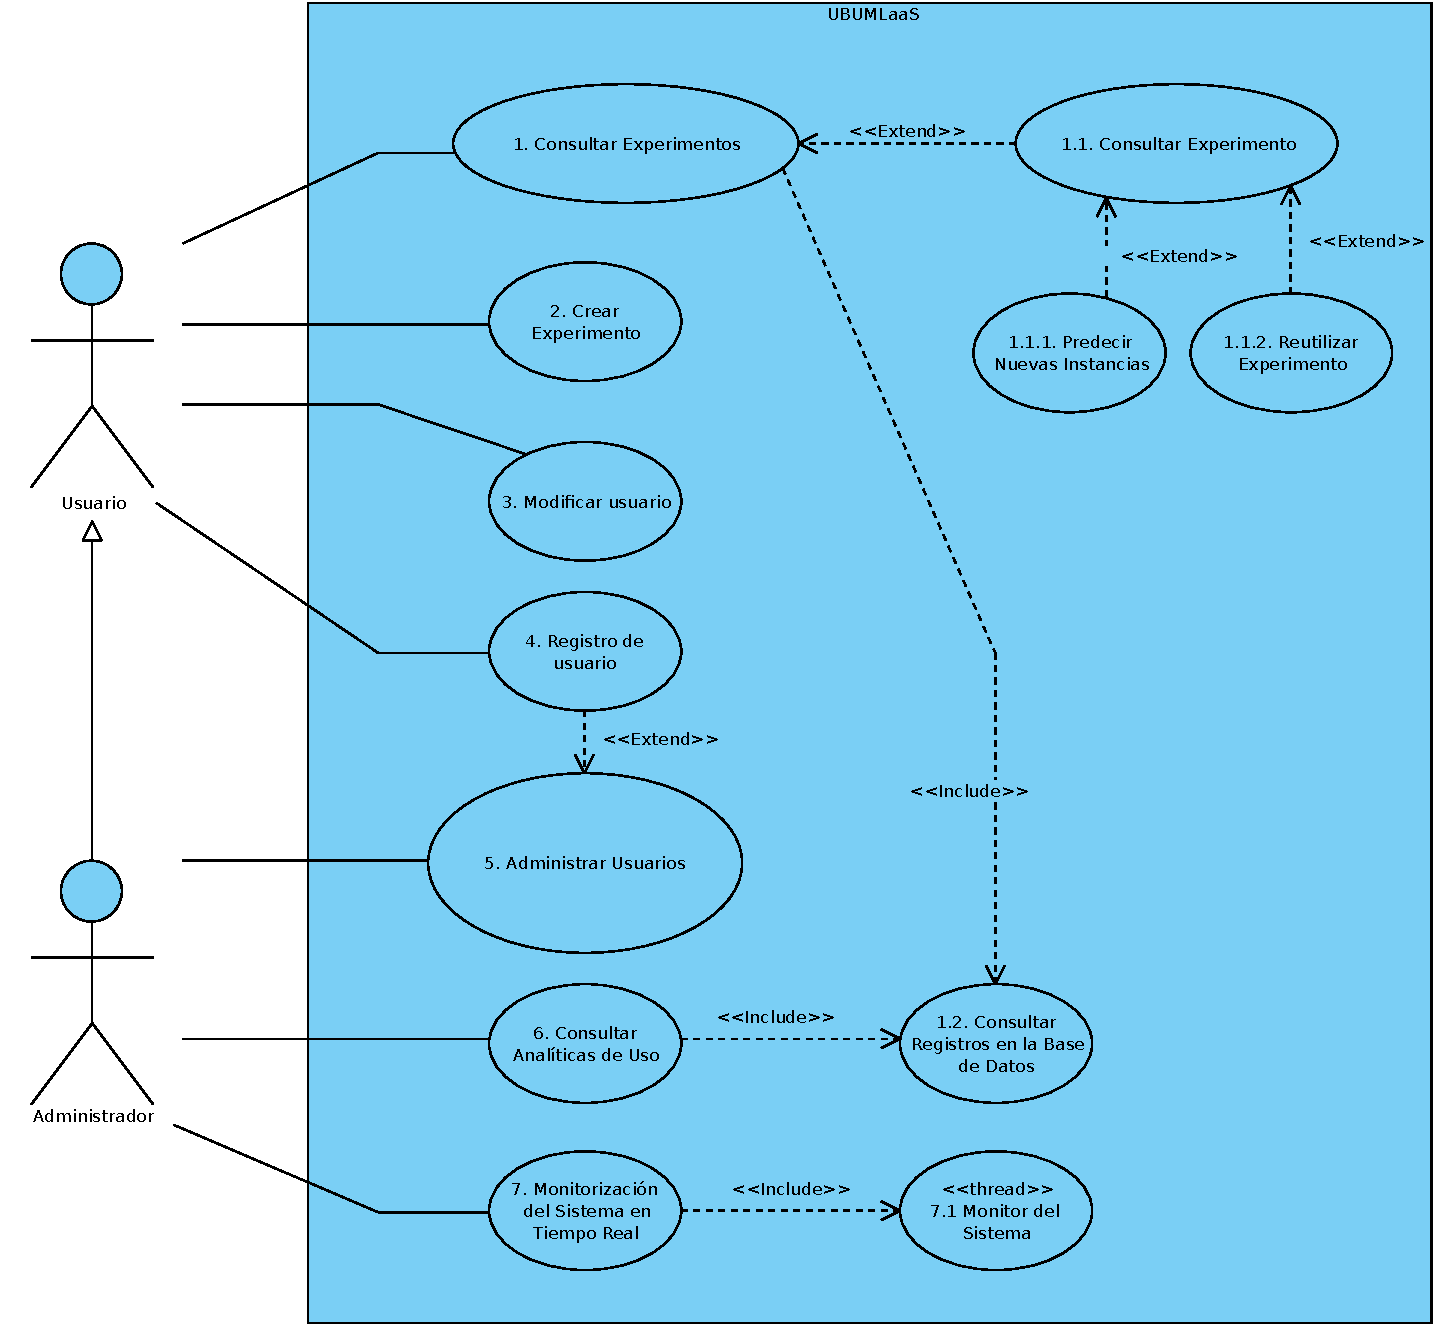
\includegraphics[scale=0.5]{../img/anexos/requisitos/Casos-de-uso}
	\caption{Diagrama de casos de uso.}\label{img:diagrama-casos-uso}
\end{figure}

\subsection{Actores}
Actuarán dos actores con el sistema, un usuario (el actor general) y un administrador (actor especializado heredado del usuario).

\subsection{Casos de uso}\label{casos-de-uso}

% Caso de Uso 1 -> Consultar Experimentos.
\begin{longtable}[H]{@{}ll@{}}
\toprule
\begin{minipage}[b]{0.23\columnwidth}\raggedright\strut
\textbf{CU-1}\strut
\end{minipage} & \begin{minipage}[b]{0.71\columnwidth}\raggedright\strut
\textbf{Consultar Experimentos}\strut
\end{minipage}\tabularnewline
\midrule
\endhead
\begin{minipage}[t]{0.23\columnwidth}\raggedright\strut
\textbf{Versión}\strut
\end{minipage} & \begin{minipage}[t]{0.71\columnwidth}\raggedright\strut
1.0\strut
\end{minipage}\tabularnewline
\begin{minipage}[t]{0.23\columnwidth}\raggedright\strut
\textbf{Autor}\strut
\end{minipage} & \begin{minipage}[t]{0.71\columnwidth}\raggedright\strut
Daniel Puente Ramírez\strut
\end{minipage}\tabularnewline
\begin{minipage}[t]{0.23\columnwidth}\raggedright\strut
\textbf{Requisitos asociados}\strut
\end{minipage} & \begin{minipage}[t]{0.71\columnwidth}\raggedright\strut
RF-1.3, RF-1.5, RF-1.6\strut
\end{minipage}\tabularnewline
\begin{minipage}[t]{0.23\columnwidth}\raggedright\strut
\textbf{Descripción}\strut
\end{minipage} & \begin{minipage}[t]{0.71\columnwidth}\raggedright\strut
Permite al usuario consultar sus experimentos y reutilizarlos.\strut
\end{minipage}\tabularnewline
\begin{minipage}[t]{0.23\columnwidth}\raggedright\strut
\textbf{Precondición}\strut
\end{minipage} & \begin{minipage}[t]{0.71\columnwidth}\raggedright\strut
El sistema de colas se encuentra en ejecución.\strut
\end{minipage}\tabularnewline
\begin{minipage}[t]{0.23\columnwidth}\raggedright\strut
\textbf{Acciones}\strut
\end{minipage} & \begin{minipage}[t]{0.71\columnwidth}\raggedright\strut
\begin{enumerate}
\def\labelenumi{\arabic{enumi}.}
\tightlist
\item El usuario entra en la plataforma.
\item Hace \textit{click} en <<Mis Experimentos>>.
\item Por cada experimento lanzado se da la opción de ver detalle, reutilizar o eliminar.
\end{enumerate}\strut
\end{minipage}\tabularnewline
\begin{minipage}[t]{0.23\columnwidth}\raggedright\strut
\textbf{Postcondición}\strut
\end{minipage} & \begin{minipage}[t]{0.71\columnwidth}\raggedright\strut
El número de experimentos mostrados al usuario es igual al número de experimentos asociados con ese ID en la base de datos.\strut
\end{minipage}\tabularnewline
\begin{minipage}[t]{0.23\columnwidth}\raggedright\strut
\textbf{Excepciones}\strut
\end{minipage} & \begin{minipage}[t]{0.71\columnwidth}\raggedright\strut
No existen excepciones posibles.\strut
\end{minipage}\tabularnewline
\begin{minipage}[t]{0.23\columnwidth}\raggedright\strut
\textbf{Importancia}\strut
\end{minipage} & \begin{minipage}[t]{0.71\columnwidth}\raggedright\strut
Alta\strut
\end{minipage}\tabularnewline
\bottomrule
\caption{CU-1 Consultar Experimentos.}
\end{longtable}

% Caso de Uso 1.1 -> Consultar Experimento
\begin{longtable}[H]{@{}ll@{}}
\toprule
\begin{minipage}[b]{0.23\columnwidth}\raggedright\strut
\textbf{CU-1.1}\strut
\end{minipage} & \begin{minipage}[b]{0.71\columnwidth}\raggedright\strut
\textbf{Consultar Experimento}\strut
\end{minipage}\tabularnewline
\midrule
\endhead
\begin{minipage}[t]{0.23\columnwidth}\raggedright\strut
\textbf{Versión}\strut
\end{minipage} & \begin{minipage}[t]{0.71\columnwidth}\raggedright\strut
1.0\strut
\end{minipage}\tabularnewline
\begin{minipage}[t]{0.23\columnwidth}\raggedright\strut
\textbf{Autor}\strut
\end{minipage} & \begin{minipage}[t]{0.71\columnwidth}\raggedright\strut
Daniel Puente Ramírez\strut
\end{minipage}\tabularnewline
\begin{minipage}[t]{0.23\columnwidth}\raggedright\strut
\textbf{Requisitos asociados}\strut
\end{minipage} & \begin{minipage}[t]{0.71\columnwidth}\raggedright\strut
RF-1.2, RF-1.3, RF-1.4, RF-1.5\strut
\end{minipage}\tabularnewline
\begin{minipage}[t]{0.23\columnwidth}\raggedright\strut
\textbf{Descripción}\strut
\end{minipage} & \begin{minipage}[t]{0.71\columnwidth}\raggedright\strut
Permite al usuario consultar un experimento en concreto, si ha finalizado, junto con las métricas reportadas.\strut
\end{minipage}\tabularnewline
\begin{minipage}[t]{0.23\columnwidth}\raggedright\strut
\textbf{Precondiciones}\strut
\end{minipage} & \begin{minipage}[t]{0.71\columnwidth}\raggedright\strut
\begin{itemize}
\tightlist
\item El experimento existe.
\item En caso de haber finalizado y tener métricas de rendimiento, se cargan.
\end{itemize}\strut
\end{minipage}\tabularnewline
\begin{minipage}[t]{0.23\columnwidth}\raggedright\strut
\textbf{Acciones}\strut
\end{minipage} & \begin{minipage}[t]{0.71\columnwidth}\raggedright\strut
\begin{enumerate}
\def\labelenumi{\arabic{enumi}.}
\tightlist
\item El usuario entra en la plataforma.
\item Hace \textit{click} en <<Mis Experimentos>>.
\item Por cada experimento lanzado se da la opción de ver detalle, reutilizar o eliminar.
\item Dentro de ver en detalle puede predecir nuevas instancias o descargar el modelo, así como consultar las métricas resultantes. En caso de haber fallado se muestra el motivo del fallo.
\end{enumerate}\strut
\end{minipage}\tabularnewline
\begin{minipage}[t]{0.23\columnwidth}\raggedright\strut
\textbf{Postcondición}\strut
\end{minipage} & \begin{minipage}[t]{0.71\columnwidth}\raggedright\strut
El identificador del experimento no varía independientemente de lo que el usuario haga con él.\strut
\end{minipage}\tabularnewline
\begin{minipage}[t]{0.23\columnwidth}\raggedright\strut
\textbf{Excepciones}\strut
\end{minipage} & \begin{minipage}[t]{0.71\columnwidth}\raggedright\strut
No existen excepciones posibles.\strut
\end{minipage}\tabularnewline
\begin{minipage}[t]{0.23\columnwidth}\raggedright\strut
\textbf{Importancia}\strut
\end{minipage} & \begin{minipage}[t]{0.71\columnwidth}\raggedright\strut
Media\strut
\end{minipage}\tabularnewline
\bottomrule
\caption{CU-1.1 Consultar Experimento.}
\end{longtable}

% Caso de Uso 1.1.1 -> Predecir Nuevas Instancias
\begin{longtable}[H]{@{}ll@{}}
\toprule
\begin{minipage}[b]{0.23\columnwidth}\raggedright\strut
\textbf{CU-1.1.1}\strut
\end{minipage} & \begin{minipage}[b]{0.71\columnwidth}\raggedright\strut
\textbf{Predecir Nuevas Instancias}\strut
\end{minipage}\tabularnewline
\midrule
\endhead
\begin{minipage}[t]{0.23\columnwidth}\raggedright\strut
\textbf{Versión}\strut
\end{minipage} & \begin{minipage}[t]{0.71\columnwidth}\raggedright\strut
1.0\strut
\end{minipage}\tabularnewline
\begin{minipage}[t]{0.23\columnwidth}\raggedright\strut
\textbf{Autor}\strut
\end{minipage} & \begin{minipage}[t]{0.71\columnwidth}\raggedright\strut
Daniel Puente Ramírez\strut
\end{minipage}\tabularnewline
\begin{minipage}[t]{0.23\columnwidth}\raggedright\strut
\textbf{Requisitos asociados}\strut
\end{minipage} & \begin{minipage}[t]{0.71\columnwidth}\raggedright\strut
RF-1.4\strut
\end{minipage}\tabularnewline
\begin{minipage}[t]{0.23\columnwidth}\raggedright\strut
\textbf{Descripción}\strut
\end{minipage} & \begin{minipage}[t]{0.71\columnwidth}\raggedright\strut
Permite al usuario predecir nuevas instancias en función a un modelo previamente entrenado.\strut
\end{minipage}\tabularnewline
\begin{minipage}[t]{0.23\columnwidth}\raggedright\strut
\textbf{Precondiciones}\strut
\end{minipage} & \begin{minipage}[t]{0.71\columnwidth}\raggedright\strut
\begin{itemize}
\tightlist
\item El experimento existe y ha finalizado.
\item Las nuevas instancias a predecir tienen los mismos atributos que con las que se entrenó el modelo.
\end{itemize}\strut
\end{minipage}\tabularnewline
\begin{minipage}[t]{0.23\columnwidth}\raggedright\strut
\textbf{Acciones}\strut
\end{minipage} & \begin{minipage}[t]{0.71\columnwidth}\raggedright\strut
\begin{enumerate}
\def\labelenumi{\arabic{enumi}.}
\tightlist
\item El usuario entra en la plataforma.
\item Hace \textit{click} en <<Mis Experimentos>>.
\item Por cada experimento lanzado se da la opción de ver detalle, reutilizar o eliminar.
\item Dentro de ver en detalle hace \textit{click} en <<Predict>>.
\item Sube el conjunto de datos a predecir.
\item Se le muestra al usuario el resultado de la predicción.
\end{enumerate}\strut
\end{minipage}\tabularnewline
\begin{minipage}[t]{0.23\columnwidth}\raggedright\strut
\textbf{Postcondición}\strut
\end{minipage} & \begin{minipage}[t]{0.71\columnwidth}\raggedright\strut
El modelo no se ha visto afectado por el proceso de predicción.\strut
\end{minipage}\tabularnewline
\begin{minipage}[t]{0.23\columnwidth}\raggedright\strut
\textbf{Excepciones}\strut
\end{minipage} & \begin{minipage}[t]{0.71\columnwidth}\raggedright\strut
El conjunto de datos pasado no cumple con los requisitos para el modelo.\strut
\end{minipage}\tabularnewline
\begin{minipage}[t]{0.23\columnwidth}\raggedright\strut
\textbf{Importancia}\strut
\end{minipage} & \begin{minipage}[t]{0.71\columnwidth}\raggedright\strut
Alta\strut
\end{minipage}\tabularnewline
\bottomrule
\caption{CU-1.1.1 Predecir Nuevas Instancias.}
\end{longtable}

% Caso de Uso 1.1.2 -> Reutilizar Experimento
\begin{longtable}[H]{@{}ll@{}}
\toprule
\begin{minipage}[b]{0.23\columnwidth}\raggedright\strut
\textbf{CU-1.1.1}\strut
\end{minipage} & \begin{minipage}[b]{0.71\columnwidth}\raggedright\strut
\textbf{Reutilizar Experimento}\strut
\end{minipage}\tabularnewline
\midrule
\endhead
\begin{minipage}[t]{0.23\columnwidth}\raggedright\strut
\textbf{Versión}\strut
\end{minipage} & \begin{minipage}[t]{0.71\columnwidth}\raggedright\strut
1.0\strut
\end{minipage}\tabularnewline
\begin{minipage}[t]{0.23\columnwidth}\raggedright\strut
\textbf{Autor}\strut
\end{minipage} & \begin{minipage}[t]{0.71\columnwidth}\raggedright\strut
Daniel Puente Ramírez\strut
\end{minipage}\tabularnewline
\begin{minipage}[t]{0.23\columnwidth}\raggedright\strut
\textbf{Requisitos asociados}\strut
\end{minipage} & \begin{minipage}[t]{0.71\columnwidth}\raggedright\strut
RF-1, RF-1.1, RF-1.1.1, RF-1.1.2, RF-1.1.3, RF-1.3\strut
\end{minipage}\tabularnewline
\begin{minipage}[t]{0.23\columnwidth}\raggedright\strut
\textbf{Descripción}\strut
\end{minipage} & \begin{minipage}[t]{0.71\columnwidth}\raggedright\strut
Permite al usuario reutilizar el experimento que ya había creado.\strut
\end{minipage}\tabularnewline
\begin{minipage}[t]{0.23\columnwidth}\raggedright\strut
\textbf{Precondiciones}\strut
\end{minipage} & \begin{minipage}[t]{0.71\columnwidth}\raggedright\strut
El experimento base existe.\strut
\end{minipage}\tabularnewline
\begin{minipage}[t]{0.23\columnwidth}\raggedright\strut
\textbf{Acciones}\strut
\end{minipage} & \begin{minipage}[t]{0.71\columnwidth}\raggedright\strut
\begin{enumerate}
\def\labelenumi{\arabic{enumi}.}
\tightlist
\item El usuario entra en la plataforma.
\item Hace \textit{click} en <<Mis Experimentos>>.
\item Busca el experimento del que desea obtener la parametrización para uno nuevo.
\item Hace \textit{click} en <<Reuse>>.
\end{enumerate}\strut
\end{minipage}\tabularnewline
\begin{minipage}[t]{0.23\columnwidth}\raggedright\strut
\textbf{Postcondición}\strut
\end{minipage} & \begin{minipage}[t]{0.71\columnwidth}\raggedright\strut
\begin{enumerate}
\tightlist
\item El modelo base no se ha visto afectado.
\item El usuario se encuentra en la pantalla <<Nuevo Experimento>> con la configuración <<nueva>>.
\end{enumerate}\strut
\end{minipage}\tabularnewline
\begin{minipage}[t]{0.23\columnwidth}\raggedright\strut
\textbf{Excepciones}\strut
\end{minipage} & \begin{minipage}[t]{0.71\columnwidth}\raggedright\strut
\begin{itemize}
\tightlist
\item Algún parámetro interno ha cambiado y ya no se puede reutilizar el experimento.
\item Solo se puede recuperar parte de la configuración.
\end{itemize}\strut
\end{minipage}\tabularnewline
\begin{minipage}[t]{0.23\columnwidth}\raggedright\strut
\textbf{Importancia}\strut
\end{minipage} & \begin{minipage}[t]{0.71\columnwidth}\raggedright\strut
Media\strut
\end{minipage}\tabularnewline
\bottomrule
\caption{CU-1.1.2 Reutilizar Experimento.}
\end{longtable}

% Caso de Uso 2 -> Crear Experimento
\begin{longtable}[H]{@{}ll@{}}
\toprule
\begin{minipage}[b]{0.23\columnwidth}\raggedright\strut
\textbf{CU-2}\strut
\end{minipage} & \begin{minipage}[b]{0.71\columnwidth}\raggedright\strut
\textbf{Crear Experimento}\strut
\end{minipage}\tabularnewline
\midrule
\endhead
\begin{minipage}[t]{0.23\columnwidth}\raggedright\strut
\textbf{Versión}\strut
\end{minipage} & \begin{minipage}[t]{0.71\columnwidth}\raggedright\strut
1.0\strut
\end{minipage}\tabularnewline
\begin{minipage}[t]{0.23\columnwidth}\raggedright\strut
\textbf{Autor}\strut
\end{minipage} & \begin{minipage}[t]{0.71\columnwidth}\raggedright\strut
Daniel Puente Ramírez\strut
\end{minipage}\tabularnewline
\begin{minipage}[t]{0.23\columnwidth}\raggedright\strut
\textbf{Requisitos asociados}\strut
\end{minipage} & \begin{minipage}[t]{0.71\columnwidth}\raggedright\strut
RF-1, RF-1.1, RF-1.1.1, RF-1.1.2, RF-1.1.3, RF-2, RF-2.1\strut
\end{minipage}\tabularnewline
\begin{minipage}[t]{0.23\columnwidth}\raggedright\strut
\textbf{Descripción}\strut
\end{minipage} & \begin{minipage}[t]{0.71\columnwidth}\raggedright\strut
Permite al usuario crear un nuevo experimento.\strut
\end{minipage}\tabularnewline
\begin{minipage}[t]{0.23\columnwidth}\raggedright\strut
\textbf{Precondiciones}\strut
\end{minipage} & \begin{minipage}[t]{0.71\columnwidth}\raggedright\strut
La parametrización es correcta.\strut
\end{minipage}\tabularnewline
\begin{minipage}[t]{0.23\columnwidth}\raggedright\strut
\textbf{Acciones}\strut
\end{minipage} & \begin{minipage}[t]{0.71\columnwidth}\raggedright\strut
\begin{enumerate}
\def\labelenumi{\arabic{enumi}.}
\tightlist
\item El usuario entra en la plataforma.
\item Hace \textit{click} en <<Nuevo Experimento>>.
\item Rellena el formulario en función de un conjunto de datos y una técnica de aprendizaje automático.
\item Hace \textit{click} en <<Crear>>.
\end{enumerate}\strut
\end{minipage}\tabularnewline
\begin{minipage}[t]{0.23\columnwidth}\raggedright\strut
\textbf{Postcondición}\strut
\end{minipage} & \begin{minipage}[t]{0.71\columnwidth}\raggedright\strut
\begin{enumerate}
\tightlist
\item El experimento ha sido añadido a las colas de ejecución.
\item El usuario recibe un correo electrónico con la finalización del experimento.
\end{enumerate}\strut
\end{minipage}\tabularnewline
\begin{minipage}[t]{0.23\columnwidth}\raggedright\strut
\textbf{Excepciones}\strut
\end{minipage} & \begin{minipage}[t]{0.71\columnwidth}\raggedright\strut
El experimento ha sido incorrectamente parametrizado y se ha levantado una excepción al intentar ejecutarlo.\strut
\end{minipage}\tabularnewline
\begin{minipage}[t]{0.23\columnwidth}\raggedright\strut
\textbf{Importancia}\strut
\end{minipage} & \begin{minipage}[t]{0.71\columnwidth}\raggedright\strut
Alta\strut
\end{minipage}\tabularnewline
\bottomrule
\caption{CU-2 Crear Experimento.}
\end{longtable}

% Caso de Uso 3 -> Modificar Usuario
\begin{longtable}[H]{@{}ll@{}}
\toprule
\begin{minipage}[b]{0.23\columnwidth}\raggedright\strut
\textbf{CU-3}\strut
\end{minipage} & \begin{minipage}[b]{0.71\columnwidth}\raggedright\strut
\textbf{Modificar Usuario}\strut
\end{minipage}\tabularnewline
\midrule
\endhead
\begin{minipage}[t]{0.23\columnwidth}\raggedright\strut
\textbf{Versión}\strut
\end{minipage} & \begin{minipage}[t]{0.71\columnwidth}\raggedright\strut
1.0\strut
\end{minipage}\tabularnewline
\begin{minipage}[t]{0.23\columnwidth}\raggedright\strut
\textbf{Autor}\strut
\end{minipage} & \begin{minipage}[t]{0.71\columnwidth}\raggedright\strut
Daniel Puente Ramírez\strut
\end{minipage}\tabularnewline
\begin{minipage}[t]{0.23\columnwidth}\raggedright\strut
\textbf{Requisitos asociados}\strut
\end{minipage} & \begin{minipage}[t]{0.71\columnwidth}\raggedright\strut
RF-4, RF-4.1, RF-4.2, RF-4.3, RF-4.4\strut
\end{minipage}\tabularnewline
\begin{minipage}[t]{0.23\columnwidth}\raggedright\strut
\textbf{Descripción}\strut
\end{minipage} & \begin{minipage}[t]{0.71\columnwidth}\raggedright\strut
Permite al usuario modificar sus datos personales dentro de la plataforma.\strut
\end{minipage}\tabularnewline
\begin{minipage}[t]{0.23\columnwidth}\raggedright\strut
\textbf{Precondiciones}\strut
\end{minipage} & \begin{minipage}[t]{0.71\columnwidth}\raggedright\strut
Los datos del usuarios son recuperados de la base de datos.\strut
\end{minipage}\tabularnewline
\begin{minipage}[t]{0.23\columnwidth}\raggedright\strut
\textbf{Acciones}\strut
\end{minipage} & \begin{minipage}[t]{0.71\columnwidth}\raggedright\strut
\begin{enumerate}
\def\labelenumi{\arabic{enumi}.}
\tightlist
\item El usuario entra en la plataforma.
\item Hace \textit{click} en <<Mis Experimentos>>.
\item Hace \textit{click} en <<Editar Perfil>>.
\item Modifica los datos como considere oportuno.
\item Hace \textit{click} en <<Guardar>>.
\end{enumerate}\strut
\end{minipage}\tabularnewline
\begin{minipage}[t]{0.23\columnwidth}\raggedright\strut
\textbf{Postcondición}\strut
\end{minipage} & \begin{minipage}[t]{0.71\columnwidth}\raggedright\strut
\begin{enumerate}
\tightlist
\item Todos los campos son validados de forma que individualmente cumplan sus respectivas restricciones de formato.
\item Para aquellos campos que deben ser únicos, se garantiza su unicidad.
\item Los datos actualizados son visibles desde el momento en el que se actualiza la página para el usuario.
\end{enumerate}\strut
\end{minipage}\tabularnewline
\begin{minipage}[t]{0.23\columnwidth}\raggedright\strut
\textbf{Excepciones}\strut
\end{minipage} & \begin{minipage}[t]{0.71\columnwidth}\raggedright\strut
Modificación concurrente en la base de datos.\strut
\end{minipage}\tabularnewline
\begin{minipage}[t]{0.23\columnwidth}\raggedright\strut
\textbf{Importancia}\strut
\end{minipage} & \begin{minipage}[t]{0.71\columnwidth}\raggedright\strut
Baja\strut
\end{minipage}\tabularnewline
\bottomrule
\caption{CU-3 Modificar Usuario.}
\end{longtable}

% Caso de Uso 4 -> Registro de Usuario
\begin{longtable}[H]{@{}ll@{}}
\toprule
\begin{minipage}[b]{0.23\columnwidth}\raggedright\strut
\textbf{CU-4}\strut
\end{minipage} & \begin{minipage}[b]{0.71\columnwidth}\raggedright\strut
\textbf{Registro de Usuario}\strut
\end{minipage}\tabularnewline
\midrule
\endhead
\begin{minipage}[t]{0.23\columnwidth}\raggedright\strut
\textbf{Versión}\strut
\end{minipage} & \begin{minipage}[t]{0.71\columnwidth}\raggedright\strut
1.0\strut
\end{minipage}\tabularnewline
\begin{minipage}[t]{0.23\columnwidth}\raggedright\strut
\textbf{Autor}\strut
\end{minipage} & \begin{minipage}[t]{0.71\columnwidth}\raggedright\strut
Daniel Puente Ramírez\strut
\end{minipage}\tabularnewline
\begin{minipage}[t]{0.23\columnwidth}\raggedright\strut
\textbf{Requisitos asociados}\strut
\end{minipage} & \begin{minipage}[t]{0.71\columnwidth}\raggedright\strut
RF-3, RF-3.1, RF-3.1.1, RF-3.1.2\strut
\end{minipage}\tabularnewline
\begin{minipage}[t]{0.23\columnwidth}\raggedright\strut
\textbf{Descripción}\strut
\end{minipage} & \begin{minipage}[t]{0.71\columnwidth}\raggedright\strut
Permite al administrador crear un nuevo usuario, o a un cliente registrarse en la plataforma y convertirse en administrador.\strut
\end{minipage}\tabularnewline
\begin{minipage}[t]{0.23\columnwidth}\raggedright\strut
\textbf{Precondiciones}\strut
\end{minipage} & \begin{minipage}[t]{0.71\columnwidth}\raggedright\strut
No existen precondiciones.\strut
\end{minipage}\tabularnewline
\begin{minipage}[t]{0.23\columnwidth}\raggedright\strut
\textbf{Acciones} (para el administrador)\strut
\end{minipage} & \begin{minipage}[t]{0.71\columnwidth}\raggedright\strut
\begin{enumerate}
\def\labelenumi{\arabic{enumi}.}
\tightlist
\item El administrador entra en la plataforma.
\item Hace \textit{click} en <<Usuarios>> en el panel lateral de administración.
\item Hace \textit{click} en <<Nuevo Usuario>>.
\item Introduce los datos del nuevo usuario.
\item Hace \textit{click} en <<Guardar>>.
\end{enumerate}\strut
\end{minipage}\tabularnewline
\begin{minipage}[t]{0.23\columnwidth}\raggedright\strut
\textbf{Postcondición}\strut
\end{minipage} & \begin{minipage}[t]{0.71\columnwidth}\raggedright\strut
\begin{enumerate}
\tightlist
\item Todos los campos son validados de forma que individualmente cumplan sus respectivas restricciones de formato.
\item Para aquellos campos que deben ser únicos, se garantiza su unicidad.
\item El nuevo usuario recibe un correo electrónico con el \textit{token} de activación de la cuenta.
\end{enumerate}\strut
\end{minipage}\tabularnewline
\begin{minipage}[t]{0.23\columnwidth}\raggedright\strut
\textbf{Excepciones}\strut
\end{minipage} & \begin{minipage}[t]{0.71\columnwidth}\raggedright\strut
Modificación concurrente en la base de datos.\strut
\end{minipage}\tabularnewline
\begin{minipage}[t]{0.23\columnwidth}\raggedright\strut
\textbf{Importancia}\strut
\end{minipage} & \begin{minipage}[t]{0.71\columnwidth}\raggedright\strut
Baja\strut
\end{minipage}\tabularnewline
\bottomrule
\caption{CU-4 Registro de Usuario.}
\end{longtable}

% Caso de Uso 5 -> Administrar Usuarios
\begin{longtable}[H]{@{}ll@{}}
\toprule
\begin{minipage}[b]{0.23\columnwidth}\raggedright\strut
\textbf{CU-5}\strut
\end{minipage} & \begin{minipage}[b]{0.71\columnwidth}\raggedright\strut
\textbf{Administrar Usuarios}\strut
\end{minipage}\tabularnewline
\midrule
\endhead
\begin{minipage}[t]{0.23\columnwidth}\raggedright\strut
\textbf{Versión}\strut
\end{minipage} & \begin{minipage}[t]{0.71\columnwidth}\raggedright\strut
1.0\strut
\end{minipage}\tabularnewline
\begin{minipage}[t]{0.23\columnwidth}\raggedright\strut
\textbf{Autor}\strut
\end{minipage} & \begin{minipage}[t]{0.71\columnwidth}\raggedright\strut
Daniel Puente Ramírez\strut
\end{minipage}\tabularnewline
\begin{minipage}[t]{0.23\columnwidth}\raggedright\strut
\textbf{Requisitos asociados}\strut
\end{minipage} & \begin{minipage}[t]{0.71\columnwidth}\raggedright\strut
RF-3, RF-3.1, RF-3.1.1, RF-3.1.2, RF-3.2, RF-3.3, RF-3.4, RF-3.5\strut
\end{minipage}\tabularnewline
\begin{minipage}[t]{0.23\columnwidth}\raggedright\strut
\textbf{Descripción}\strut
\end{minipage} & \begin{minipage}[t]{0.71\columnwidth}\raggedright\strut
Permite al administrador crear, (de)activar, hacer (o quitar de) administrador, o eliminar a un usuario.\strut
\end{minipage}\tabularnewline
\begin{minipage}[t]{0.23\columnwidth}\raggedright\strut
\textbf{Precondiciones}\strut
\end{minipage} & \begin{minipage}[t]{0.71\columnwidth}\raggedright\strut
El usuario a modificar no es el mismo usuario que está modificando.\strut
\end{minipage}\tabularnewline
\begin{minipage}[t]{0.23\columnwidth}\raggedright\strut
\textbf{Acciones} (para el administrador)\strut
\end{minipage} & \begin{minipage}[t]{0.71\columnwidth}\raggedright\strut
\begin{enumerate}
\def\labelenumi{\arabic{enumi}.}
\tightlist
\item El administrador entra en la plataforma.
\item Hace \textit{click} en <<Usuarios>> en el panel lateral de administración.
\item Puede buscar si así lo desea al usuario en cuestión.
\item Realiza las modificaciones pertinentes.
\end{enumerate}\strut
\end{minipage}\tabularnewline
\begin{minipage}[t]{0.23\columnwidth}\raggedright\strut
\textbf{Postcondición}\strut
\end{minipage} & \begin{minipage}[t]{0.71\columnwidth}\raggedright\strut
La modificación ha sido correcta.\strut
\end{minipage}\tabularnewline
\begin{minipage}[t]{0.23\columnwidth}\raggedright\strut
\textbf{Excepciones}\strut
\end{minipage} & \begin{minipage}[t]{0.71\columnwidth}\raggedright\strut
Modificación concurrente en la base de datos.\strut
\end{minipage}\tabularnewline
\begin{minipage}[t]{0.23\columnwidth}\raggedright\strut
\textbf{Importancia}\strut
\end{minipage} & \begin{minipage}[t]{0.71\columnwidth}\raggedright\strut
Media\strut
\end{minipage}\tabularnewline
\bottomrule
\caption{CU-5 Administrar Usuarios.}
\end{longtable}

% Caso de Uso 6 -> Consultar Analíticas de Uso
\begin{longtable}[H]{@{}ll@{}}
\toprule
\begin{minipage}[b]{0.23\columnwidth}\raggedright\strut
\textbf{CU-6}\strut
\end{minipage} & \begin{minipage}[b]{0.71\columnwidth}\raggedright\strut
\textbf{Consultar Analíticas de Uso}\strut
\end{minipage}\tabularnewline
\midrule
\endhead
\begin{minipage}[t]{0.23\columnwidth}\raggedright\strut
\textbf{Versión}\strut
\end{minipage} & \begin{minipage}[t]{0.71\columnwidth}\raggedright\strut
1.0\strut
\end{minipage}\tabularnewline
\begin{minipage}[t]{0.23\columnwidth}\raggedright\strut
\textbf{Autor}\strut
\end{minipage} & \begin{minipage}[t]{0.71\columnwidth}\raggedright\strut
Daniel Puente Ramírez\strut
\end{minipage}\tabularnewline
\begin{minipage}[t]{0.23\columnwidth}\raggedright\strut
\textbf{Requisitos asociados}\strut
\end{minipage} & \begin{minipage}[t]{0.71\columnwidth}\raggedright\strut
RF-6, RF-6.1, RF-6.1.1, RF-6.1.2, RF-6.1.3, RF-6.2, RF-6.2.1, RF-6.2.2, RF-6.2.3\strut
\end{minipage}\tabularnewline
\begin{minipage}[t]{0.23\columnwidth}\raggedright\strut
\textbf{Descripción}\strut
\end{minipage} & \begin{minipage}[t]{0.71\columnwidth}\raggedright\strut
Permite a un usuario comprobar sus estadísticas de uso. Y si es administrador, las del la plataforma.\strut
\end{minipage}\tabularnewline
\begin{minipage}[t]{0.23\columnwidth}\raggedright\strut
\textbf{Precondiciones}\strut
\end{minipage} & \begin{minipage}[t]{0.71\columnwidth}\raggedright\strut
Existen estadísticas que mostrar.\strut
\end{minipage}\tabularnewline
\begin{minipage}[t]{0.23\columnwidth}\raggedright\strut
\textbf{Acciones} (para el usuario)\strut
\end{minipage} & \begin{minipage}[t]{0.71\columnwidth}\raggedright\strut
\begin{enumerate}
\def\labelenumi{\arabic{enumi}.}
\tightlist
\item El usuario entra en la plataforma.
\item Hace \textit{click} en <<Mis Experimentos>>.
\item Hace \textit{click} en <<Estadísticas>>.
\item Puede visualizar las estadísticas generales de la plataforma.
\end{enumerate}\strut
\end{minipage}\tabularnewline
\begin{minipage}[t]{0.23\columnwidth}\raggedright\strut
\textbf{Acciones} (para el administrador)\strut
\end{minipage} & \begin{minipage}[t]{0.71\columnwidth}\raggedright\strut
\begin{enumerate}
\def\labelenumi{\arabic{enumi}.}
\tightlist
\item El administrador entra en la plataforma.
\item Hace \textit{click} en \textit{<<Dashboard>>} en el panel lateral de administración.
\item Puede visualizar las estadísticas generales de la plataforma.
\end{enumerate}\strut
\end{minipage}\tabularnewline
\begin{minipage}[t]{0.23\columnwidth}\raggedright\strut
\textbf{Postcondición}\strut
\end{minipage} & \begin{minipage}[t]{0.71\columnwidth}\raggedright\strut
No existen postcondiciones.\strut
\end{minipage}\tabularnewline
\begin{minipage}[t]{0.23\columnwidth}\raggedright\strut
\textbf{Excepciones}\strut
\end{minipage} & \begin{minipage}[t]{0.71\columnwidth}\raggedright\strut
No existen excepciones.\strut
\end{minipage}\tabularnewline
\begin{minipage}[t]{0.23\columnwidth}\raggedright\strut
\textbf{Importancia}\strut
\end{minipage} & \begin{minipage}[t]{0.71\columnwidth}\raggedright\strut
Alta\strut
\end{minipage}\tabularnewline
\bottomrule
\caption{CU-6 Consultar Analíticas de Uso.}
\end{longtable}

% Caso de Uso 7 -> Monitorización del Sistema en Tiempo Real
\begin{longtable}[H]{@{}ll@{}}
\toprule
\begin{minipage}[b]{0.23\columnwidth}\raggedright\strut
\textbf{CU-7}\strut
\end{minipage} & \begin{minipage}[b]{0.71\columnwidth}\raggedright\strut
\textbf{Monitorización del Sistema en Tiempo Real}\strut
\end{minipage}\tabularnewline
\midrule
\endhead
\begin{minipage}[t]{0.23\columnwidth}\raggedright\strut
\textbf{Versión}\strut
\end{minipage} & \begin{minipage}[t]{0.71\columnwidth}\raggedright\strut
1.0\strut
\end{minipage}\tabularnewline
\begin{minipage}[t]{0.23\columnwidth}\raggedright\strut
\textbf{Autor}\strut
\end{minipage} & \begin{minipage}[t]{0.71\columnwidth}\raggedright\strut
Daniel Puente Ramírez\strut
\end{minipage}\tabularnewline
\begin{minipage}[t]{0.23\columnwidth}\raggedright\strut
\textbf{Requisitos asociados}\strut
\end{minipage} & \begin{minipage}[t]{0.71\columnwidth}\raggedright\strut
RF-5, RF-5.1, RF-5.2, RF-5.3\strut
\end{minipage}\tabularnewline
\begin{minipage}[t]{0.23\columnwidth}\raggedright\strut
\textbf{Descripción}\strut
\end{minipage} & \begin{minipage}[t]{0.71\columnwidth}\raggedright\strut
Permite al administrador comprobar el estado de carga actual del sistema.\strut
\end{minipage}\tabularnewline
\begin{minipage}[t]{0.23\columnwidth}\raggedright\strut
\textbf{Precondiciones}\strut
\end{minipage} & \begin{minipage}[t]{0.71\columnwidth}\raggedright\strut
Existen registros de datos para calcular las estadísticas que mostrar.\strut
\end{minipage}\tabularnewline
\begin{minipage}[t]{0.23\columnwidth}\raggedright\strut
\textbf{Acciones}\strut
\end{minipage} & \begin{minipage}[t]{0.71\columnwidth}\raggedright\strut
\begin{enumerate}
\def\labelenumi{\arabic{enumi}.}
\tightlist
\item El administrador entra en la plataforma.
\item Hace \textit{click} en \textit{<<Live Monitor>>} en el panel lateral de administración.
\item Puede visualizar las estadísticas generales de la plataforma.
\end{enumerate}\strut
\end{minipage}\tabularnewline
\begin{minipage}[t]{0.23\columnwidth}\raggedright\strut
\textbf{Postcondición}\strut
\end{minipage} & \begin{minipage}[t]{0.71\columnwidth}\raggedright\strut
No existen postcondiciones.\strut
\end{minipage}\tabularnewline
\begin{minipage}[t]{0.23\columnwidth}\raggedright\strut
\textbf{Excepciones}\strut
\end{minipage} & \begin{minipage}[t]{0.71\columnwidth}\raggedright\strut
Si no existen datos que mostrar aún.\strut
\end{minipage}\tabularnewline
\begin{minipage}[t]{0.23\columnwidth}\raggedright\strut
\textbf{Importancia}\strut
\end{minipage} & \begin{minipage}[t]{0.71\columnwidth}\raggedright\strut
Alta\strut
\end{minipage}\tabularnewline
\bottomrule
\caption{CU-7 Monitorización del Sistema en Tiempo Real.}
\end{longtable}

% Caso de Uso 7.1 -> Monitor del Sitema
\begin{longtable}[H]{@{}ll@{}}
\toprule
\begin{minipage}[b]{0.23\columnwidth}\raggedright\strut
\textbf{CU-7.1}\strut
\end{minipage} & \begin{minipage}[b]{0.71\columnwidth}\raggedright\strut
\textbf{Monitor del Sitema}\strut
\end{minipage}\tabularnewline
\midrule
\endhead
\begin{minipage}[t]{0.23\columnwidth}\raggedright\strut
\textbf{Versión}\strut
\end{minipage} & \begin{minipage}[t]{0.71\columnwidth}\raggedright\strut
1.0\strut
\end{minipage}\tabularnewline
\begin{minipage}[t]{0.23\columnwidth}\raggedright\strut
\textbf{Autor}\strut
\end{minipage} & \begin{minipage}[t]{0.71\columnwidth}\raggedright\strut
Daniel Puente Ramírez\strut
\end{minipage}\tabularnewline
\begin{minipage}[t]{0.23\columnwidth}\raggedright\strut
\textbf{Requisitos asociados}\strut
\end{minipage} & \begin{minipage}[t]{0.71\columnwidth}\raggedright\strut
RF-5.1, RF-5.2, RF-5.3\strut
\end{minipage}\tabularnewline
\begin{minipage}[t]{0.23\columnwidth}\raggedright\strut
\textbf{Descripción}\strut
\end{minipage} & \begin{minipage}[t]{0.71\columnwidth}\raggedright\strut
Proceso de recolección de información de uso del sistema.\strut
\end{minipage}\tabularnewline
\begin{minipage}[t]{0.23\columnwidth}\raggedright\strut
\textbf{Precondiciones}\strut
\end{minipage} & \begin{minipage}[t]{0.71\columnwidth}\raggedright\strut
Glances está instalado en el sistema.\strut
\end{minipage}\tabularnewline
\begin{minipage}[t]{0.23\columnwidth}\raggedright\strut
\textbf{Acciones}\strut
\end{minipage} & \begin{minipage}[t]{0.71\columnwidth}\raggedright\strut
Ninguna, ejecución en paralelo en el sistema.\strut
\end{minipage}\tabularnewline
\begin{minipage}[t]{0.23\columnwidth}\raggedright\strut
\textbf{Postcondición}\strut
\end{minipage} & \begin{minipage}[t]{0.71\columnwidth}\raggedright\strut
No existen postcondiciones.\strut
\end{minipage}\tabularnewline
\begin{minipage}[t]{0.23\columnwidth}\raggedright\strut
\textbf{Excepciones}\strut
\end{minipage} & \begin{minipage}[t]{0.71\columnwidth}\raggedright\strut
No existen excepciones.\strut
\end{minipage}\tabularnewline
\begin{minipage}[t]{0.23\columnwidth}\raggedright\strut
\textbf{Importancia}\strut
\end{minipage} & \begin{minipage}[t]{0.71\columnwidth}\raggedright\strut
Alta\strut
\end{minipage}\tabularnewline
\bottomrule
\caption{CU-7.1 Monitor del Sitema.}
\end{longtable}
\apendice{Especificación de diseño}

\section{Introducción}
En este anexo se va a exponer cómo se han resuelto los objetivos anteriormente comentados. Así como la definición de datos que se utilizan en la aplicación, procedimientos, etc. 

\section{UBUMLaaS}
\subsection{Diseño de datos}
La aplicación cuenta con las siguientes entidades:
\begin{itemize}
\item \textbf{Usuarios (Users).} Posee toda la información relacionada con los usuarios. Almacenando su identificador único en el sistema, su correo electrónico, usuario, contraseña \textit{hasheada}, país y uso que ha indicado que va a dar a ala aplicación, además de si se encuentra activo o no, o del tipo de usuario que es (administrador o usuario normal). 

Como campos adicionales puede almacenar la página web del usuario, algunas redes sociales como son Twitter, LinkedIn, GitHub. Junto con la institución a la que pertenece y su Google Scholar.

\item \textbf{Algoritmos (Algorithms).} Guarda la información relacionada con cada algoritmo que se puede utilizar, teniendo un identificador único, un nombre de algoritmo para uso interno, el nombre que se mostrará en la web, así como los parámetros de configuración y a qué biblioteca pertenece.

\item \textbf{Filtros (Filters).} Guarda la información relacionada con cada filtro que se puede utilizar, teniendo un identificador único, un nombre de filtro para uso interno, el nombre que se mostrará en la web, así como los parámetros de configuración y a qué biblioteca pertenece.

\item \textbf{Experimentos (Experiments).} Almacena toda la información de un experimento lanzado. Posee un identificador de experimento único, el identificador del usuario que lo lanzó, el nombre (interno) del algoritmo en cuestión, junto con la configuración de este, y forma homónima para los filtros (en caso de utilizar un filtro).  Referencia a los datos de entrenamiento, y en caso de haber terminado, los resultados del experimento. 

Posee dos \textit{timestamps} representando la hora de inicio y fin del entrenamiento, un campo adicional representa el estado que tiene. Junto con todos estos datos se almacena la configuración del experimento.

\item \textbf{Países (Countries).} Recoge toda la información que puede ser útil a la hora de trabajar con países. Posee el nombre oficial del país en cuestión, así como la representación en \texttt{Alpha 2}\footnote{Los códigos alfa-2 son códigos de dos letras definidos en la norma ISO 3166-1, utilizados para designar países territorios independientes y zonas geográficas especiales. Son utilizados principalmente en los dominios geográficos de primer nivel en Internet, además de direcciones postales.} y \texttt{3}, el número de identificación único de cada país, además, la longitud y latitud de la capital del país. 
\end{itemize}

\clearpage
\begin{landscape}
\subsubsection{Diagrama E/R}
\imagenAncho{../img/anexos/design/ERD-C}{Diagrama entidad relación.}{erd}{1.30}
\end{landscape}

\subsubsection{Diagrama Relacional}
\imagenRuta{../img/anexos/design/relational}{Diagrama relacional.}{relational}
\FloatBarrier

\subsection{Diseño procedimental}
En esta sección interna se recogen los detalles más relevantes en cuanto a los procedimientos llevados a cabo por la plataforma en función de las acciones del usuario.

A continuación se explican los diagramas de secuencia (DS):
\begin{itemize}
\item \textbf{DS para la monitorización del sistema en tiempo real.} Figura~\ref{fig:DSec-LiveMonitor}. Muestra el proceso seguido por el sistema en el momento en el que solicita la vista correspondiente. Es el único diagrama en el que se muestra la comprobación de si es administrador o no, por brevedad en el resto se indica en forma de texto nada más. 

Cuando el sistema recoge la solicitud de visualización busca los datos necesarios en la base de datos, y en el caso de no haber pasado todavía 10 minutos (valor umbral) del inicio del sistema, buscará un fichero de histórico en el que se guardan los últimos 6 meses de datos como máximo. Se procesan los datos ya que existen muchos más de los que el sistema mostrará y se devolverá la página HTML.

\item \textbf{DS para las estadísticas generales (System Analytics).} Figura~\ref{fig:DSec-SystemAnalytics}. Necesita privilegios de administrador, omitido en el diagrama por claridad. Debido a la multitud de operaciones que debe se deben realizar, posee una pantalla de carga que se muestra al usuario en lo que es sistema prepara la visualización. 

Internamente se recorre prácticamente la base de datos en su totalidad y se obtienen las estadísticas correspondientes. En el momento en el que se tienen todos los valores calculados se guardarán en ficheros temporales que se leerán y al poco tiempo un recolector de basura los eliminará.

\item \textbf{DS para crear un experimento.} Figura~\ref{fig:DSec-NewExpUser}. Cuando un usuario accede a la vista de crear un nuevo experimento, prácticamente cada botón y desplegable tienen repercusión directa en el sistema. 

En la elección/subida de un conjunto de datos, se harán operaciones de lectura/escritura respectivamente sobre un directorio específico en el que se encuentran almacenados. 

Para la selección de algoritmos y filtros, una vez se selecciona el tipo de algoritmo a utilizar, se leen de la base de datos aquellos algoritmos y filtros compatibles y se muestran al usuario para su elección. Una vez seleccionados se renderizan los parámetros de configuración particulares de cada uno de ellos.

Finalmente, el usuario mandará crear el experimento, pasando al lado del servidor la ejecución de este, ver Figura~\ref{fig:DSec-NewExpServer}.

\item \textbf{DS para la ejecución de un experimento.} Figura~\ref{fig:DSec-NewExpServer}. En el momento en el que el usuario manda crear el experimento, se le muestra la pantalla en la cual aparecerán los resultados, pero con un GIF indicando que aún no ha terminado la ejecución. 

El servidor recoge la configuración indicada por el usuario para realizar el experimento y lo encola en las colas de ejecución \texttt{high-ubumlaas}, en las que cuándo estén disponibles, realizarán el experimento según la configuración recibida. 

En el momento en el que el experimento finalice, la cola pasará a ejecutar el siguiente experimento (de existir), y se le devolverá el control al sistema, este último se encargará de almacenar los resultados en la entrada correspondiente al experimento en la base de datos, de tal manera que cuando el usuario proceda a ver los resultados pueda visualizarlos. Finalmente mandará un correo electrónico al usuario <<dueño>> del experimento indicando que ha finalizado.

\end{itemize}

\clearpage
\imagenRuta{../img/anexos/design/DSec-LiveMonitor.pdf}{Diagrama de secuencia de la monitorización en tiempo real.}{DSec-LiveMonitor}
\imagenRuta{../img/anexos/design/DSec-SystemAnalytics.pdf}{Diagrama de secuencia de las estadísticas generales de la aplicación.}{DSec-SystemAnalytics}
\imagenFlotante{../img/anexos/design/DSec-NewExpUser.pdf}{Diagrama de secuencia de la creación de un nuevo experimento por parte del usuario.}{DSec-NewExpUser}
\begin{landscape}
\imagenAncho{../img/anexos/design/DSec-NewExpServer.pdf}{Diagrama de secuencia de la ejecución de un nuevo experimento.}{DSec-NewExpServer}{1.5}
\end{landscape}

\subsection{Diseño arquitectónico}
\imagenFlotante{../img/anexos/design/client-server}{Arquitectura cliente-servidor.}{client-server}
La aplicación con el fin de cumplir con todos los requerimientos funcionales así como objetivos principales, y por ende, conseguir un bajo acoplamiento y una alta cohesión. Sigue una arquitectura de cliente servidor.

En la Figura~\ref{fig:client-server} se aprecia un modelo simplificado de la arquitectura seguida, en la cual los procesos se van a dividir en dos grupos. 
\begin{itemize}
\item Servidor. Implementa el servicio de \texttt{UBUMLaaS}.
\item Cliente. Solicitará los servicios de proporcionados por el servidor.
\end{itemize}

\subsubsection{Arquitectura de tres capas}
La aplicación sigue una arquitectura de tres capas (multicapa), siguiendo esta arquitectura el cliente implementa la lógica de presentación (es un cliente ligero); el servidor de aplicación implementa la lógica de negocio, y los datos residen en una base de datos de \texttt{SQLite}, por definición de la arquitectura de tres capas sería necesario que hubiera un servidor dedicado a la comunicación con la base de datos, pero ahí es donde reside una de las cualidades de \texttt{SQLite}, es \textit{serverless}, permitiendo una auto-gestión y soportando múltiples clientes realizando tareas en paralelo.

UBUMLaaS sigue esta arquitectura por las siguientes razones:
\begin{itemize}
\item Desacoplamiento, cambios en la interfaz de usuario o en la lógica de la aplicación son independientes entre sí, favoreciendo la evolución de la aplicación hacia nuevos requerimientos.
\item Se minimizan los cuellos de botella de la red, la información transmitida es únicamente la solicitada.
\item El cliente está separado (aislado) de la base de datos, pudiendo acceder de manera sencilla a los recursos sin necesidad de conocer la ubicación de los datos.
\end{itemize}

\FloatBarrier
%%%%%%%%%%%%%%%%%%%%%%%%%%%%%%%%%%%%%%%%%%%%%%%%%%%%%%%%%%%%
\section{IS-SSL}
\subsection{Diseño de datos}
En esta sección se van a seleccionar las representaciones lógicas de los datos, las estructuras de datos utilizadas.

Los algoritmos implementados se encuentran divididos en dos bibliotecas, la separación se realiza en base al criterio lógico de qué hacen los algoritmos de cada una de ellas. Por un lado, están los algoritmos de selección de instancias, y por el otro, los algoritmos de aprendizaje semi-supervisado.

Todos los algoritmos utilizan la clase auxiliar \textit{Nearest Neighbors} de Scikit-Learn~\cite{NearestNeighbors} para el cálculo de los vecinos cercanos. Teniendo en cuenta que la distancia a sí misma es cero, se han codificado los algoritmos para evitar que un prototipo posea como vecino más cercano a sí mismo.

\subsection{Diseño procedimental}
A continuación, se recogen los detalles para poder hacer uso de los algoritmos.

Todos los algoritmos se pueden utilizar de la misma manera que se esperaría al utilizar los propios de la biblioteca de Scikit-Learn. Por lo tanto, una vez están importados los correspondientes se utilizarán:
\begin{itemize}
\item Algoritmos de selección de instancias.
\begin{enumerate}
	\item Instanciar el objeto a utilizar, pasando los parámetros de configuración deseados.
	\item Pasar el conjunto de datos al método \texttt{filter} del modelo.
	\item Recoger los resultados.
\end{enumerate}
\item Algoritmos de aprendizaje semi-supervisado.
\begin{enumerate}
\item Instanciar el objeto a utilizar, pasando los parámetros de configuración, así como referencias a algoritmos de clasificación si no se quieren utilizar los proporcionados <<por defecto>>.
\item Pasar al método \texttt{fit} el conjunto de datos, indicando aquellas instancias para las que no se conoce la clase, con su clase a -1.
\item Pasar al método \texttt{predict} el conjunto de datos a predecir. Obteniendo las etiquetas para el conjunto de datos pasado.
\end{enumerate}
\end{itemize}

\textbf{NOTA.} Todas las entradas son objetos de tipo \texttt{DataFrame} de la biblioteca \texttt{Pandas}. Las salidas cuándo son vectores de una dimensión, son \textit{arrays} de \texttt{NumPy}, si son de más de una dimensión, \texttt{DataFrames}.

\subsection{Diseño arquitectónico}
Debido a que se trata de una serie de bibliotecas de algoritmos, no son lo suficientemente grandes como para aplicar patrones de diseño los cuales proporcionen algún tipo de ventaja significativa. 

\subsubsection{Diseño en paquetes}
Para la organización de los diferentes archivos que componen las bibliotecas se ha seguido la estrategia de \textit{package per feature approach} (paquete por característica).

Esta estrategia permite agrupar todos los archivos en función de la funcionalidad que aportan, aumentando la legibilidad del árbol de paquetes, su modularización, así como su desarrollo continuo y ampliación de algoritmos soportados.

Ambas bibliotecas incluyen el directorio interno de \texttt{utils}. El cual proporciona clases y métodos necesarios, comunes a varios algoritmos de la biblioteca principal. 

\apendice{Documentación técnica de programación}

\section{Introducción}
En este anexo se va a describir con detalle la documentación técnica de programación. Se describirá la estructura de directorios que posee, la instalación del propio entorno de desarrollo, cómo llevar a cabo su compilación, instalación y ejecución; además de las pruebas que se han realizado.

Se debe recordar que el proyecto se encuentra dividido en dos repositorios diferenciados, UBUMLaaS e IS-SSL\footnote{Biblioteca de algoritmos de selección de instancias y aprendizaje semi-supervisado programado.}; es por ello que, se dividirá en dos secciones respectivamente, y tantas subsecciones como son necesarias para cada uno de ellos.

\section{UBUMLaaS}

\subsection{Estructura de directorios}
La estructura del repositorio es la siguiente:
\begin{itemize}
\tightlist
\item \texttt{/}: raíz del proyecto, aquí se encuentra el README, la licencia, los ficheros de configuración de las pruebas de integración y despliegue continuo (CI-CD), junto con los ficheros de requisitos para \texttt{conda} y \texttt{pyenv}. 
\item \texttt{/lib/}: librerías utilizadas por el sistema.
\item \texttt{/lib/is\_ssl}: librería propia de métodos de selección de instancias y aprendizaje semi-supervisado.
\item \texttt{/lib/scikit\_ml\_learn\_data/meka/meka-release-1.9.2/}: librería \texttt{Meka} en su versión 1.9.2.
\item \texttt{/lib/skmultilearn/}: librería \texttt{scikit-multilearn}.
\item \texttt{/lib/unofficial\_weka\_packages/}: algoritmos de ADMIRABLE.
\item \texttt{/lib/wekafiles/}: algoritmos concretos de \texttt{weka}.
\item \texttt{/test/*}: ficheros de prueba CI-CD.
\item \texttt{/ubumlaas/}: directorio principal de la plataforma.
\item \texttt{/ubumlaas/admin/}: contiene toda la parte de \textit{backend} de administración.
\item \texttt{/ubumlaas/core/}: contiene el \textit{backend} de las vistas de índice y acerca de.
\item \texttt{/ubumlaas/default\_datasets/}: conjuntos de datos por defecto que se añaden a los nuevos usuarios.
\item \texttt{/ubumlaas/error\_pages/}: contiene el \textit{backend} de las vistas de error.
\item \texttt{/ubumlaas/experiments/}: contiene el \textit{backend} para la realización de experimentos.
\item \texttt{/ubumlaas/experiments/algorithm/}: contiene las métricas para el análisis del modelo entrenado.
\item \texttt{/ubumlaas/experiments/execute\_algorithm/}: contiene opciones de ejecución para cada librería.
\item \texttt{/ubumlaas/experiments/views/}: control de las vistas relacionadas con los experimentos.
\item \texttt{/ubumlaas/jobs/}: descripción de \textit{RQ Worker Builder}.
\item \texttt{/ubumlaas/static/}: contiene los ficheros estáticos de la plataforma.
\item \texttt{/ubumlaas/static/avatars/}: contiene las imágenes de perfil de cada usuario.
\item \texttt{/ubumlaas/static/css/}: contiene el código \texttt{CSS} del \textit{frontend}.
\item \texttt{/ubumlaas/static/img/}: contiene las imágenes que aparecen en la pltaforma.
\item \texttt{/ubumlaas/static/js/}: contiene el código \texttt{JavaScript} del \textit{frontend}.
\item \texttt{/ubumlaas/templates/}: ficheros \texttt{HTML}.
\item \texttt{/ubumlaas/templates/admin/}: ficheros web de administración.
\item \texttt{/ubumlaas/templates/blocks/}: ficheros web de bloques que se añaden sobre otros documentos web.
\item \texttt{/ubumlaas/templates/error\_pages/}: ficheros web de errores (403, 404, \dots)
\item \texttt{/ubumlaas/templates/modals/}: ficheros para la representación de modales.
\item \texttt{/ubumlaas/users/}: contiene el \textit{backend} de las actividades relacionadas con el usuario.
\item \texttt{/ubumlaas/weka/}: contiene los ficheros de configuración de \texttt{Weka} y su \texttt{VM}.

\end{itemize}

\subsection{Manual del programador}
En esta subsección se describen todos aquellos recursos seguidos por el equipo de desarrollo para, valga la redundancia, desarrollar el proyecto. De tal forma que un futuro desarrollador/mantenedor del proyecto no tenga inconvenientes a la hora de retomar el proyecto y conocerlo.

\subsubsection{Entorno de desarrollo}
Para poder continuar con el desarrollo del proyecto, se requiere tener instalado el siguiente \textit{software} en el equipo:
\begin{itemize}
\tightlist
\item Python 3.7+.
\item Bibliotecas Python.
\item Git
\item VSCode
\end{itemize}

En los siguientes apartados se detalla la instalación de cada uno de los componentes anteriormente citados.

\subsubsection{Python 3.7+}
Al comienzo del proyecto, muchas de sus funcionalidades eran compatibles con Python 2, pero el nuevo desarrollo ha utilizado indistintamente métodos existentes en versiones anteriores de Python y algunos que se han introducido a partir de la version 3.7, disponible desde~\cite{pythonGetIt}. Es importante que los binarios se encuentren en el \texttt{path} del sistema para que no de problemas de ejecución.

\subsubsection{Bibliotecas Python}
A continuación (ver Tabla~\ref{tab:bibliotecas-python-ubumlaas}), se van a detallar uno de los puntos más importantes para poder <<hacer funcionar>> el proyecto, puesto que se van a necesitar versiones concretas de determinadas librerías para que todo se integre correctamente con todo y se pueda ver y utilizar como un sistema homogéneo.

\begin{table}[p]
\centering
\begin{tabular}{lcl}
	\textbf{Biblioteca} & \textbf{Versión} & \textbf{Descripción}\\
	\toprule
	\rowcolor[HTML]{EFEFEF} 
	\texttt{email-validator} & 1.1.1 & Validar direcciones de correo electrónico.\\
	\texttt{flask} & 1.1.1 & Web \textit{framework}.\\ \rowcolor[HTML]{EFEFEF}
	\texttt{flask-login} & 0.4.1 & Control usuarios y sesiones en Flask.\\
	\texttt{flask-mail} & 0.9.1 & Envío de \textit{emails} con Flask.\\ \rowcolor[HTML]{EFEFEF}
	\texttt{flask-migrate} & 2.5.2 & Migrar SQLAchemy DB a Flask.\\
	\texttt{flask-redis} & 0.4.0 & Soporte a Redis en Flask.\\ \rowcolor[HTML]{EFEFEF}
	\texttt{flask-sqlalchemy} & 2.4.0 & Soporte a SQLAchemy en Flask.\\
	\texttt{flask-wtf} & 0.14.2 & Render, validar y CSRF formularios.\\ \rowcolor[HTML]{EFEFEF}
	\texttt{future} & 0.16.0 & Soporte a Python 2 y 3.\\ 
	\texttt{geopy} & 2.2.0 & Geocodificación.\\ \rowcolor[HTML]{EFEFEF}
	\texttt{glances} & 3.2.4.2 & Monitorización del sistema.\\ 
	\texttt{imbalanced-learn} & 0.5.0 & ML con datos desbalanceados.\\ \rowcolor[HTML]{EFEFEF}
	\texttt{itsdangerous} & 1.1.0 & Paso de datos en entornos no seguros.\\
	\texttt{liac-arff} & 2.2.1 & Escritura y lectura de ficheros ARFF.\\ \rowcolor[HTML]{EFEFEF}
	\texttt{numpy} & 1.22.3 & Computación de \textit{arrays}.\\
	\texttt{pandas} & 0.25.1 & Estructuras de datos.\\ \rowcolor[HTML]{EFEFEF}
	\texttt{psutil} & 5.9.0 & Procesar y monitorizar sistemas.\\
	\texttt{pycountry} & 22.3.5 & Datos de países.\\ \rowcolor[HTML]{EFEFEF}
	\texttt{pytest} & 5.2.1 & Pruebas en Python.\\
	\texttt{python-weka-wrapper3} & 0.1.7 & \textit{Wrapper} para Weka.\\ \rowcolor[HTML]{EFEFEF}
	\texttt{requests} & 2.22.0 & \textit{Requests} para humanos.\\
	\texttt{rq} & 1.1.0 & Crear y procesar trabajos <<de fondo>>.\\ \rowcolor[HTML]{EFEFEF}
	\texttt{scikit-learn} & 0.24 & Módulos de minería de datos y ML.\\ 
	\texttt{selenium} & 3.141.0 & Auto interacción con navegador web.\\ \rowcolor[HTML]{EFEFEF}
	\texttt{urllib3} & 1.25.6 & Conexiones HTTP seguras.\\
	\texttt{werkzeug} & 0.15.6 & Biblioteca de aplicaciones web WSGI.\footnote{\textit{Web Server Gateway Interface.}. Es una especificación que describe cómo un servidor web se comunica con las aplicaciones web, y cómo las aplicaciones web pueden encadenarse para procesar una solicitud.}\\ \rowcolor[HTML]{EFEFEF}
	\texttt{whichcraft} & 0.4.1 & Funcionalidad \textit{shutil.which}. \\
	\bottomrule
\end{tabular}
\caption{Bibliotecas utilizadas y sus versiones.}\label{tab:bibliotecas-python-ubumlaas}
\end{table}

Las versiones indicadas en la tabla~\ref{tab:bibliotecas-python-ubumlaas} son las que se han utilizado para el desarrollo del proyecto, se pueden actualizar a versiones futuras, siempre y cuando sean compatibles entre sí.

\subsubsection{Git}
\imagenRuta{../img/anexos/manual-programador/gitkraken}{Interfaz de \texttt{GitKraken}.}{gitkraken}
Para poder utilizar el repositorio ha de utilizarse el gestor de versiones \texttt{Git}. Se recomienda utilizar GUI con soporte a VC\footnote{Control de versiones (\textit{Version Control}).} tales que no requieran de una interfaz de comandos para su utilización, pero eso se deja a decisión del futuro desarrollador.

En la Figura~\ref{fig:gitkraken} se aprecia como el \textit{software} \texttt{GitKraken} permite, de forma intuitiva y sencilla, el uso de \texttt{Git} y todo su potencial. Se puede obtener desde~\cite{gitkraken}.

El repositorio posee una serie diferente de ramas de trabajo, se recomienda para producción utilizar o el último \textit{release} o bien la rama principal.

\subsubsection{Visual Studio Code}
\texttt{Visual Studio Code} es una herramienta de amplia versatilidad la cual soporta todos los lenguajes de programación utilizados en este proyecto (y muchos más) de forma nativa; además, posee ciertos \textit{plugins} que facilitan el desarrollo proporcionando \textit{snippets} y similares. Se recomienda su uso ya que es un IDE <<todo-en-uno>>, facilitando las tareas de desarrollo. 

Se puede obtener desde~\cite{VSCode}.

\subsection{Compilación, instalación y ejecución del proyecto}
En esta subsección se va a detallar el proceso a seguir para poder hacer uso del proyecto en local, modificarlo y/o utilizarlo. La forma de desarrollo del proyecto no ha sido estrictamente en local, sino que el proyecto se encontraba alojado en un equipo servidor y mediante SSH\footnote{\textit{Suite} de protocolos los cuales especifican estándares para operar los servicios de red de forma segura entre anfitriones para los que no existe una relación de confianza a través de redes no seguras. Las comunicaciones entre pares se encuentran encriptadas.} se realizaba la conexión y posterior edición de los ficheros.

\subsubsection{Adquisición del código fuente}
Lo primero que se necesita es obtener el código en el equipo, para ello podemos seguir una de las siguientes aproximaciones:
\begin{itemize}
\item Mediante el uso de la terminal.
\begin{enumerate}
\tightlist
\item Apertura de la terminal.
\item Desplazarse al directorio en donde se desee clonar el repositorio (usando \texttt{cd} en Unix o \texttt{dir} en Windows).
\item Hacer uso del siguiente comando:\\
\texttt{git clone https://github.com/dpr1005/UBUMLaaS.git}
\item Se dispone de una copia idéntica a la alojada en el repositorio de \texttt{GitHub}.
\end{enumerate}

\item Descarga desde el navegador.
\begin{itemize}
\tightlist
\item Apertura del navegador preferido.
\item Introducir en la barra de búsqueda la siguiente dirección:\\
\texttt{https://github.com/dpr1005/UBUMLaaS/archive/refs/\\heads/master.zip}
\item Aceptar la descarga en caso de tener habilitada la comprobación.
\item Navegar con el Explorador de archivos del sistema hasta el directorio de descarga.
\end{itemize}

\item Uso de \texttt{GitKraken}.
\begin{itemize}
\tightlist
\item Apertura de la aplicación.
\item Hacer \textit{click} en \textit{Clone a repo}.
\item En \textit{Repository Management} $\rightarrow$ \textit{Clone} $\rightarrow$ \textit{Clone with URL}: 
\begin{itemize}
\item Indicar la ruta local en la que nos interesa que se clone el repositorio.
\item En URL introducir:\\
\texttt{git clone https://github.com/dpr1005/UBUMLaaS.git}
\end{itemize}
\item Hacer \textit{click} en \textit{Clone the repo!}.
\end{itemize}
\end{itemize}

\subsubsection{Importar el proyecto en Visual Studio Code}
Se diferencian dos aproximaciones, local o como se ha operado, conexión mediante SSH.

\begin{itemize}
\item Importar el proyecto en la propia máquina donde se va a desplegar y será en ella en la que se edite.
\begin{enumerate}
\item Apertura de \texttt{Visual Studio Code}.
\item Hacer \textit{click} en Abrir.
\item Seleccionar el directorio raíz dónde lo hayamos alojado.
\end{enumerate}
\item Importar el proyecto en una máquina y editarlo desde otra.
\begin{enumerate}
\item Seguir los pasos de la adquisición del código en la máquina en la que se va a alojar el código. En el equipo local no va a estar.
\item Apertura de \texttt{Visual Studio Code}
\item Navegar a las Extensiones e instalar \texttt{Remote - SSH}, disponible desde~\cite{VSCode-Remote-SSH}.
\item Instalar un cliente SSH compatible con \texttt{OpenSSH}. Ver guía~\cite{Remote-Development-Tricks-Tips}.
\item Con todo instalado, se realiza la conexión a la máquina remota.
\begin{enumerate}
\item Presionar \texttt{F1} y correr el comando: \texttt{Remote-SSH: Open SSH Host...}
\item Introducir el usuario y el \texttt{host/IP} en el formato:\\
\texttt{user@host-o-ip} ó \texttt{user@domain@host-o-ip}
\item En caso de que se solicite, introducir la contraseña, pero se recomienda configurar el uso de llaves SSH, ver guía~\cite{Remote-Development-Tricks-Tips}.
\item Después de la conexión usar Archivo $\rightarrow$ Abrir carpeta, para abrir el directorio donde se encuentra el proyecto en la máquina remota.
\end{enumerate}
\item Todos los cambios que se realicen, se harán sobre el código en la máquina remota, la máquina local no hará más que el efecto de editor.
\end{enumerate}
\end{itemize}

\subsubsection{Crear entorno virtual de trabajo}
Para poder trabajar con este proyecto (independientemente de si es para desarrollo o producción) hacen falta una serie de bibliotecas concretas de Python, las cuales, como es lógico, deben estar en la máquina en la que se va a correr; dicho con otras palabras, en la que está el código. El proyecto está preparado para crear un entorno de \texttt{Conda} propio, de forma que no interfiera con otros proyectos y sea más sencillo de mantener y actualizar.

Se recomienda que los binarios de anaconda o miniconda estén configurados en el \texttt{path} del sistema para poder utilizar el comando \texttt{conda} desde la línea de comandos.

El proceso de creación del entrono virtual con \texttt{Conda} es el siguiente:
\begin{enumerate}
\tightlist
\item Apertura de la terminal.
\item Navegar hasta la raíz del proyecto.
\item Crear el entorno con:\\
\texttt{conda env create -f UBUMLaaS\_env.yml}
\item Cuando se desee utilizar se debe activar:\\
\texttt{conda activate UBUMLaaS}
\end{enumerate}

También se puede utilizar el procedimiento habitual para importar las bibliotecas al actual \texttt{venv} de la sesión de la terminal, pero se desaconseja su uso ya que un entorno <<genérico>> antes o después se actualizará por otros proyectos, pudiendo generar incompatibilidades con el proyecto UBUMLaaS.

\subsubsection{Instalación en Linux}
Con los anteriores pasos realizados, la importación del proyecto y la activación del entorno virtual, se deben modificar una serie de ficheros con el fin de habilitar todas las funcionalidades que ofrece el proyecto. 

Se deben seguir los siguientes pasos:
\begin{enumerate}
\item Modificar \texttt{env\_variables.sh} con los valores correctos para cada uno de los campos:
\begin{lstlisting}[language=bash]
export SECRET_KEY=<app secret key>
export EMAIL_AC=<email>
export EMAIL_PASS=<email-password>
export EMAIL_URL=<email-url>
export FLASK_ENV=development #development or production
LIBFOLDER=/absolute/path/to/UBUMLaaS
\end{lstlisting}
\item Dentro del entorno virtual de UBUMLaaS en \texttt{Conda}, se debe ejecutar el siguiente comando para permitir la importación de las variables anteriormente declaradas al entorno virtual.\\
\texttt{source env\_vars\_to\_conda.sh}
\item Creación de la base de datos.\\
\texttt{mv data\_base.sqlite ubumlaas/data.sqlite}\\
* En caso de poseer una base de datos con la configuración correcta, se puede poner en \texttt{./ubumlaas/} bajo el nombre de \texttt{data.sqlite}.
\item En caso de no tener instalado y configurado \texttt{Redis-Server}, ejecutar:
\begin{lstlisting}[language=bash]
sudo apt install redis-server
sudo service redis-server start
sudo systemctl enable redis-server
\end{lstlisting}
\end{enumerate}

\subsubsection{Uso del proyecto}
Lo primero de todo para poder tener el producto trabajando, es desplegarlo, para ello es requisito haber completado todos los pasos previos de esta sección. Activar el entorno virtual de \texttt{Conda}, correr el lanzador, y ya está en ejecución.
\begin{lstlisting}[language=bash]
conda activate UBUMLaaS
./run.sh
\end{lstlisting}
\textbf{Nota.} Es importante asegurarnos que todos los ficheros de las librerías y el lanzador del proyecto poseen permisos de ejecución necesarios (en instalaciones <<por defecto>> de Debian, CentOS, SUSE, no debería de ser necesario más que dar permisos de ejecución al lanzador).

El usuario administrador por defecto es \texttt{Admin@AdminUBUMLaaS.es} y su contraseña es \texttt{admin4123!UBUMLaaS}.

\subsection{Integración Continua}
Con el objetivo de obtener como producto final un \textit{software} de calidad, se han desarrollado una serie de pruebas de integración continua, las cuales se comprueban y analiza su resultado en cada \textit{commit} y/o \textit{pull request.}

Se han utilizado principalmente tres herramientas \textit{cloud} para medir los principios de calidad del \textit{software}.

\subsubsection{Codacy}
Herramienta la cual proporciona soporte a análisis automático del código fuente e identifica los problemas a medida que avanza. Su versatilidad permite desarrollar \textit{software} de manera eficiente, reduciendo el número de \textit{bugs} que se <<dejan para resolver>>. 

A través del análisis estático de código estático, notifica problemas de seguridad, cobertura del código, así como la duplicación y la complejidad de cada fichero en cada \textit{commit} y \textit{pull request}.

\imagenRuta{../img/anexos/manual-programador/Codacy-UBUMLaaS}{Codacy.}{Codacy-UBUMLaaS}

\subsubsection{Sonar Cloud}
Herramienta \textit{open source} la cual permite hacer un análisis estático del código de un proyecto, entre sus fortalezas destaca su potente capacidad de ser parametrizada, entre las acciones que realiza por defecto encontramos la detección de malas prácticas, errores de código, así como problemas de seguridad que en el pasado se han visto relacionadas con alguna CVE\footnote{\textit{Common Vulnerabilities and Exposures}, lista de fallos \textit{software} (y \textit{hardware}) que en el pasado se han utilizado para ganar ventaja de alguna manera.}.

A pesar de que sea un proyecto \textit{open source} no es gratuita, y como todas las herramientas de estas características incluye una versión \textit{community} (gratuita) para aquellos proyectos que sean \textit{open source}.

\imagenRuta{../img/anexos/manual-programador/SonarCloud-UBUMLaaS}{SonarCloud.}{SonarCloud-UBUMLaaS}

\subsubsection{Travis-CI}
Herramienta \textit{cloud} desarrollada para la realización de pruebas de integración continua sobre proyectos alojados en GitHub (con soporte beta para BitBucket, Gitlab y Assembla). Permite realizar un \textit{build} del proyecto y ejecutar sobre ella una batería de pruebas de manera automática cada vez que se realiza un \textit{commit} y/o \textit{pull request}, permitiendo pruebas concurrentes, incluso sobre diferentes sistemas operativos (Linux, Windows, macOS y FreeBSD). 

Con el proyecto configurado en \texttt{Travis-CI} se debe configurar un fichero \texttt{YAML} y debe de estar en el directorio raíz, será a partir del cual se ejecuten las pruebas.

El fichero se encuentra dividido en:
\begin{itemize}
\tightlist
\item \texttt{os:} sistema/s operativo/s sobre el cuál se va/n a realizar las pruebas.
\item \texttt{dist:} distribución a utilizar.
\item \texttt{language:} lenguaje de programación del proyecto.
\item \texttt{python:} especificación de la versión de Python que necesita.
\item \texttt{node\_js:} especificación de la versión de Node JS que necesita.
\item \texttt{jdk:} especificación de la versión de JDK necesaria.
\item \texttt{jobs:} parametrización de los trabajos que se van a ejecutar.
\item \texttt{git:} profundidad del árbol de \texttt{git} que deseamos utilizar.
\item \texttt{addons:} \textit{software} <<extra>> que se necesiten para las pruebas.
\item \texttt{services:} especificación de los servicios que se van a utilizar.
\item \texttt{before\_install:} definición de comandos a ejecutar antes de los incluidos en la sección \texttt{install}.
\item \texttt{install:} definición de comandos de instalación de dependencias.
\item \texttt{before\_script:} configuración de dependencias antes de ejecutar la sección \texttt{script}.
\item \texttt{script:} pruebas a realizar.
\end{itemize}

Los \textit{logs} son públicos y consultables desde~\cite{Travis-CI-LOG-UBUMLaaS}.

\imagenRuta{../img/anexos/manual-programador/Travis-CI-UBUMLaaS}{Travis-CI.}{Travis-CI-UBUMLaaS}

\subsection{Pruebas del sistema}
Intro \\
Tal y como se ha descrito, \texttt{UBUMLaaS} es un \textit{software} que ha sufrido un cambio de diseño de grandes dimensiones, por lo que las pruebas de integración continua previas que existían han dejado de ser funcionales, debido a que únicamente comprobaban la interacción del usuario con la plataforma a través de un navegador.

\clearpage
\section{IS-SSL}

\subsection{Estructura de directorios}
La estructura del repositorio es la siguiente:
\begin{itemize}
\tightlist
\item \texttt{/}: raíz del proyecto, aquí se encuentra el README, la licencia, los ficheros de configuración de PIP, los ficheros de configuración de las pruebas de integración y despliegue continuo (CI-CD); y, el fichero de requisitos.
\item \texttt{/datasets/*}: conjuntos de datasets en formatos \texttt{csv} y \texttt{arff}, normalizados y no normalizados.
\item \texttt{/docs/}: documentación del proyecto.
\item \texttt{/docs/img/}: imágenes utilizadas en la documentación.
\item \texttt{/docs/img/anexos/*}: imágenes utilizadas en los anexos.
\item \texttt{/docs/img/draws/}: diagramas en su formato original.
\item \texttt{/docs/img/memoria/*}: imágenes utilizadas en la memoria.
\item \texttt{/hypothesis/*}: primera aproximación a la investigación realizada.
\item \texttt{/implementation\_tests/}: conjunto de pruebas de validación sobre los algoritmos implementados.
\item \texttt{/instance\_selection/}: algoritmos implementados de selección de instancias.
\item \texttt{/instance\_selection/utils/}: métodos de apoyo comunes a los algoritmos de selección de instancias.
\item \texttt{/misc/}: contiene archivos varios de formato para el repositorio (cabeceras, logos, etc.).
\item \texttt{/semisupervised/}: algoritmos implementados de aprendizaje semi-supervisado.
\item \texttt{/semisupervised/utils/}: métodos de apoyo comunes a los algoritmos de aprendizaje semi-supervisado.
\item \texttt{/utils/}: diferentes clases y métodos de apoyo comunes tanto a selección de instancias como a semi-supervisado.
\end{itemize}

\subsection{Manual del programador}
En esta subsección se describen todos aquellos métodos seguidos por el equipo de desarrollo para, valga la redundancia, desarrollar el proyecto. De tal forma que un futuro desarrollador no tenga inconvenientes a la hora de retomar el proyecto.

\subsubsection{Entorno de desarrollo}
Para poder continuar con el desarrollo del proyecto, se requiere tener instalado el siguiente \textit{software} en el equipo:
\begin{itemize}
\tightlist
\item Python 3.7+.
\item Bibliotecas Python.
\item Git
\item VSCode/PyCharm/\dots.
\end{itemize}

En los siguientes apartados se detalla la instalación de cada uno de los componentes anteriormente citados.

\subsubsection{Python 3.7+}
El desarrollo se ha realizado siguiendo las últimas formas de programación disponibles a partir de la versión 3.7 de Python. El desarrollo se comenzó después de que se dejara de mantener Python 2, por lo que se trabajó desde el inicio con versiones de Python 3. Se puede obtener la última versión disponible de Python desde~\cite{pythonGetIt}. Es importante que el desarrollador se asegure que los binarios han sido añadidos al \texttt{path} del sistema que esté utilizando.

\subsubsection{Bibliotecas Python}
Esta sección es la más importante de todas junto con la anterior, debido a que el proyecto depende de (está construido utilizando) bibliotecas de $3^{os}$. Y en especial, determinadas versiones de las mismas. 

En la Tabla~\ref{tab:bibliotecas-python-is-ssl} se detallan las bibliotecas necesarias para utilizar el proyecto tal y como se encuentra en el repositorio. Para el uso en exclusiva de las librerías de \texttt{IS-SSL} se deben utilizar aquellas que se encuentran en negrita.

\begin{table}[]
\centering
\begin{tabular}{lcl}
	\textbf{Biblioteca} & \textbf{Versión} & \textbf{Descripción}\\ \rowcolor[HTML]{EFEFEF} 
	\toprule
	\rowcolor[HTML]{EFEFEF} 
	\texttt{matplotlib}    & 3.4.3   & Representación gráfica.   \\  
	\textbf{\texttt{numpy}}    & 1.20.3 &  Computación de \textit{arrays}.  \\ \rowcolor[HTML]{EFEFEF} 
	\textbf{\texttt{pandas}}    & 1.3.4  & Estructuras de datos    \\  
	\textbf{\texttt{scikit-learn}}    & 0.24.2 & Módulos de minería de datos y ML.   \\ \rowcolor[HTML]{EFEFEF} 
	\textbf{\texttt{scipy}}    & 1.7.1  & Módulos científicos.    \\ 
	\texttt{yagmail}    & 0.15.277  & Cliente de GMAIL.    \\ 
	\bottomrule
\end{tabular}
\caption{Bibliotecas utilizadas y sus versiones.}\label{tab:bibliotecas-python-is-ssl}
\end{table}

Se recomienda el uso de un entorno de desarrollo de \texttt{Conda}, se facilitan ficheros de configuración tanto para \texttt{Conda} como para instalación con \texttt{PIP}.

\subsubsection{Git}
Para poder utilizar el repositorio ha de utilizarse el gestor de versiones \texttt{Git}. Se recomienda utilizar GUI con soporte a VC tales que no requieran de una interfaz de comandos para su utilización, pero eso se deja a decisión del futuro desarrollador.

\subsubsection{VSCode/Pycharm/\dots}
El desarrollo propio del producto puede ser realizado en cualquier editor de textos, incluso en \texttt{Vi} si así se desea. La ventaja de herramientas como \texttt{Visual Studio Code} o \texttt{PyCharm}, es que permiten el uso de \textit{plugins} añadidos a los complementos del propio IDE, lo cual permite la generación de código un proceso mucho más sencillo y directo, reduciendo el número de errores ocasionados y permitiendo una depuración o refactorización del código fuente mucho más eficiente y sencilla.

Se puede obtener cada una de las herramientas desde~\cite{VSCode, PyCharm}, respectivamente.

\subsection{Compilación, instalación y ejecución del proyecto}
En esta subsección se va a detallar el proceso a seguir para poder hacer uso del proyecto en local, modificarlo y/o utilizarlo. 

\subsubsection{Adquisición del código fuente}
Lo primero que se necesita es obtener el código en el equipo, para ello podemos seguir una de las siguientes aproximaciones:
\begin{itemize}
\item Mediante el uso de la terminal.
\begin{enumerate}
\tightlist
\item Apertura de la terminal.
\item Desplazarse al directorio en donde se desee clonar el repositorio (usando \texttt{cd} en Unix o \texttt{dir} en Windows).
\item Hacer uso del siguiente comando:\\
\texttt{git clone https://github.com/dpr1005/\\Semisupervised-learning-and-instance-selection-\\methods.git}
\item Se dispone de una copia idéntica a la alojada en el repositorio de \texttt{GitHub}.
\end{enumerate}

\item Descarga desde el navegador.
\begin{itemize}
\tightlist
\item Apertura del navegador preferido.
\item Introducir en la barra de búsqueda la siguiente dirección:\\
\texttt{https://github.com/dpr1005/\\Semisupervised-learning-and-instance-selection-methods/\\archive/refs/heads/main.zip}
\item Aceptar la descarga en caso de tener habilitada la comprobación.
\item Navegar con el Explorador de archivos del sistema hasta el directorio de descarga.
\end{itemize}

\item Uso de \texttt{GitKraken}.
\begin{itemize}
\tightlist
\item Apertura de la aplicación.
\item Hacer \textit{click} en \textit{Clone a repo}.
\item En \textit{Repository Management} $\rightarrow$ \textit{Clone} $\rightarrow$ \textit{Clone with URL}: 
\begin{itemize}
\item Indicar la ruta local en la que nos interesa que se clone el repositorio.
\item En URL introducir:\\
\texttt{git clone https://github.com/dpr1005/\\Semisupervised-learning-and-instance-selection-\\methods.git}
\end{itemize}
\item Hacer \textit{click} en \textit{Clone the repo!}.
\end{itemize}
\end{itemize}

\subsubsection{Importar el proyecto en PyCharm}
Importar un proyecto en \texttt{PyCharm} es tan sencillo como:
\begin{enumerate}
\tightlist
\item Apertura de \texttt{PyCharm}.
\item Hacer \textit{click} en \textit{Open.} (Notar que también podríamos clonar el proyecto en este momento haciendo \textit{click} en \textit{Get from VCS}).
\item Seleccionar la ruta en el equipo dónde se encuentra el directorio raíz del proyecto.
\end{enumerate}

\subsubsection{Crear entorno virtual de trabajo}
Como se ha comentado previamente, para poder trabajar con este proyecto se requieren de una serie de bibliotecas de Python. El proyecto está preparado para crear un entorno de \texttt{Conda} propio, de forma que no interfiera con otros proyectos y sea más sencillo de mantener y actualizar.

Se recomienda que los binarios de anaconda o miniconda estén configurados en el \texttt{path} del sistema para poder utilizar el comando \texttt{conda} desde la línea de comandos.

El proceso de creación del entrono virtual con \texttt{Conda} es el siguiente:
\begin{enumerate}
\tightlist
\item Apertura de la terminal.
\item Navegar hasta la raíz del proyecto.
\item Crear el entorno con:\\
\texttt{conda env create -f is-ssl.yml}
\item Cuando se desee utilizar se debe activar:\\
\texttt{conda activate is-ssl}
\end{enumerate}

En caso de que se desee añadir al entorno (\texttt{venv}) actual en el que se encuentre el usuario:
\begin{enumerate}
\tightlist
\item Apertura de la terminal.
\item Navegar hasta la raíz del proyecto.
\item Instalar los requerimientos del proyecto con:\\
\texttt{pip install -r requeriments.txt}
\end{enumerate}

\subsubsection{Uso del proyecto}
La forma de usar la biblioteca es muy sencilla, todo \texttt{IS-SSL} ha sido codificado siguiendo la misma guía de estilo (PEP 8), de forma que cualquier programador habituado con el uso de bibliotecas en Python lo encuentre intuitivo y sencillo.

Todos los métodos de selección de instancias y algoritmos de aprendizaje semi-supervisado son clases de Python, de manera que para utilizarlo hay que hacer una importación del paquete y de la clase.

Un ejemplo del uso completo de este \textit{software} es lo encontramos en Listing~\ref{lst:ejemplo}, donde se detallan los tipos de datos de entrada.

Según la codificación realizada, todos los métodos accesibles de las clases esperan la entrada de objetos de tipo \texttt{DataFrame} de la librería de \texttt{Pandas}. Internamente en función de las operaciones que tenga que realizar, serán convertidos estos objetos a listas de Python o arreglos de \texttt{NumPy}. Independientemente de las operaciones internas, siempre la salida producida (en caso de tenerla) serán objetos de \texttt{Pandas}, no teniendo que ser necesariamente el mismo objeto de entrada modificado, en la mayor parte de las ocasiones serán objetos nuevos.

\begin{lstlisting}[language=Python, caption={Ejemplo de uso de IS-SSL}, label={lst:ejemplo}]
from ssl_dnx import TriTraining
from is_dnx import ENN
from sklearn.naive_bayes import GaussianNB
from sklearn.neighbors import KNeighborsClassifier
from sklearn.tree import DecisionTreeClassifier
from sklearn.datasets import load_iris
	
if __name__ == "__main__":
	model = TriTraining(
		random_state = 42,
		c1 = GaussianNB, c1_params = None,
		c2 = KNeighborsClassifier, c2_params = {n_neighbors: 2},
		c3 = DecisionTreeClassifier, c3_params = None	
	)
	filter_model = ENN(nearest_neighbors = 5, power_parameter = 2)
	
	iris = load_iris()
	X = iris['data']
	y = iris['target']

	X = pd.DataFrame(X)
	y = pd.DataFrame(y)
	X, y = filter_model.filter(X, y)

	val = [True if i % 2 == 0 else False for i in range(len(y))]
	y[val] = -1

	X, X_test, y, y_test = train_test_split(X.to_numpy(), y.to_numpy())

	X = pd.DataFrame(X)
	y = pd.DataFrame(y)

	model.fit(X, y)
	y_pred = model.predict(X_test)
	print(accuracy_score(y_true=y_test, y_pred=y_pred))
	
\end{lstlisting}
\pagebreak

\subsection{Integración Continua}
Con el objetivo de diseñar un \textit{software} lo más robusto posible, la biblioteca cuenta con una serie de pruebas de integración continua, permitiendo que todos los cambios que se vayan realizando mantengan la biblioteca en un estado correcto, indicando tempranamente aquellos posibles problemas que puedan surgir.

Este proceso se ha divido en dos etapas, una más <<adelantada>> y otra más <<tardía>>, la principal diferencia es el objetivo perseguido con cada una de las pruebas. 
\begin{itemize}
\item Inicial. Se configuró la segunda semana de febrero, con el objetivo de comenzar a tener una visión más amplia y razonada de la calidad del código, debido a que todavía no estaban desarrollados al 100\% todos los algoritmos y aún eran susceptibles de sufrir modificaciones en tanto en cuanto a sus entradas/salidas/optimización. 
\item Posterior. Se configuró en Semana Santa, (segunda semana de abril), en esta fase se implementaron una batería de pruebas la cual cubre prácticamente la totalidad de \texttt{IS-SSL}, permitiendo obtener una base para futuras modificaciones que puedan ser necesarias realizar, asegurando que todo sigue funcionando como debería.
\end{itemize}

A pesar de que se han utilizado diferentes herramientas que se podría decir que cubren los mismos tópicos, cada una implementa las diferentes métricas de análisis de forma diferente, y por lo tanto se puede ganar en este proceso. El código cubierto no se ha configurado en cada herramienta por simplicidad, ya que ahí no hay <<medias tintas>> es un informe el que se genera y las herramientas lo único que proporcionan es un visor de ese fichero.

Los recursos utilizados para la integración continua se detallan a continuación.

\subsubsection{Codacy}
Herramienta la cual proporciona soporte a análisis automático del código fuente e identifica los problemas a medida que avanza. Su versatilidad permite desarrollar \textit{software} de manera eficiente, reduciendo el número de \textit{bugs} que se <<dejan para resolver>>. 

A través del análisis estático de código estático, notifica problemas de seguridad, cobertura del código, así como la duplicación y la complejidad de cada fichero en cada \textit{commit} y \textit{pull request}.

La integración es muy sencilla, basta con crearse una cuenta asociada con la de GitHub, y una vez que se ha verificado se añade la organización a la que se pertenece y el repositorio (público) que se desea comenzar a analizar. En caso de que el repositorio sea privado, pasados los 14 días de prueba se deberá actualizar la licencia de uso a una superior.

\imagenRuta{../img/anexos/manual-programador/Codacy-IS-SSL}{Codacy.}{Codacy-IS-SSL}

En la Figura~\ref{fig:Codacy-IS-SSL} se aprecia uno de los gráficos que muestra Codacy, en este caso referido al número de \textit{issues} detectados en el código analizado. Tal y como se muestra, se ha realizado un trabajo a lo largo del mes de febrero y marzo para obtener una librería sin fallos aumentando su mantenibiliad.

\subsubsection{Sonar Cloud}

Herramienta \textit{open source} la cual permite hacer un análisis estático del código de un proyecto, entre sus fortalezas destaca su potente capacidad de ser parametrizada, entre las acciones que realiza por defecto encontramos la detección de malas prácticas, errores de código, así como problemas de seguridad que en el pasado se han visto relacionadas con alguna CVE\footnote{\textit{Common Vulnerabilities and Exposures}, lista de fallos \textit{software} (y \textit{hardware}) que en el pasado se han utilizado para ganar ventaja de alguna manera.}.

A pesar de que sea un proyecto \textit{open source} no es gratuita, y como todas las herramientas de estas características incluye una versión \textit{community} (gratuita) para aquellos proyectos que sean \textit{open source}.

El proceso de integración es sencillo, una vez registrados y asociada la cuenta con una de GitHub, se selecciona sobre qué proyecto se desea comenzar a analizar el código. El siguiente paso es definir un conjunto de reglas (si no se quiere utilizar el que se proporciona por defecto), y en cada \textit{pull request} que se realice al repositorio, Sonar Cloud analizará todos los cambios y emitirá un informe consultable desde la web así como un comentario en la propia \textit{pull request} con los resultados encontrados.

\imagenRuta{../img/anexos/manual-programador/SonarCloud-IS-SSL}{SonarCloud.}{SonarCloud-IS-SSL}

\subsection{Pruebas del sistema}

\apendice{Documentación de usuario}

\section{Introducción}
En esta sección se detallan los requerimientos de la aplicación, su instalación y despliegue (en el caso de \texttt{UBUMLaaS}) y se acompañan de una serie de indicaciones y consejos para su correcto uso.

De igual manera que en el Manual del Programador cada parte del proyecto, \texttt{IS-SSL} y \texttt{UBUMLaaS}, se describirá por su propio lado, de tal manera que aunque haya aspectos comunes, cada una su propia documentación de usuario.

\section{UBUMLaaS}
En esta sección se va a presentar el manual de usuario para el correcto uso de la plataforma \texttt{UBUMLaaS}, de tal forma que sirva como guía para comprender y consiguientemente poder utilizar eficientemente el \textit{software} desarrollado.
\subsection{Requisitos de usuarios}
Los requisitos mínimos para poder hacer uso de \texttt{UBUMLaaS} son:
\begin{itemize}
\item Disponer de una conexión a Internet.
\item Hacer uso de navegador web con soporte a HTML5.
\item Tener habilitado JavaScript en el navegador.
\item Tener una cuenta en la plataforma.
\end{itemize}
\subsection{Instalación}
Al tratarse de un producto web no se requiere de ningún tipo de instalación. Los navegadores Google Chrome, Mozilla Firefox, Safari y Microsfot Edge son soportados\footnote{Todos ellos han sido probados por el equipo de desarrollo y usuarios encuestados a  los que se les proporcionó un documento de uso básico y lo usaron en sus dispositivos cotidianos.}, siempre y cuando se encuentren en versiones compatibles con HTML5 y tengan activado el uso de JavaScript.

Independientemente del dispositivo de uso (ordenador de sobremesa, portátil, tableta o móvil), se requiere de conexión a Internet como es lógico. Pero no necesita de permisos adicionales, ha sido desarrollada de tal manera que utiliza la sesión local del navegador sin necesidad del uso de \textit{cookies}.

Aunque se hizo un intento de traducción a los lenguajes más comunes, finalmente se encuentra en inglés de forma única.

\subsection{Manual del usuario}
En esta sección se describe como un usuario nuevo puede registrarse en la aplicación desarrollada, iniciar sesión, crear sus propios experimentos, así como predecir nuevas etiquetas con modelos ya entrenados.

\subsubsection{Registro}

Lo primero de todo una vez se conozca la URL en la que se encuentra desplegada la aplicación, es acceder a la misma, y se llegará a una página web similar a la Figura~\ref{fig:index-no-login}, pudiendo variar en función de la resolución del dispositivo (dispositivos móviles no son recomendados pero si tabletas). 

\imagenFlotante{../img/anexos/manual-usuario/UBUMLaaS/index-no-login}{Página de inicio.}{index-no-login}

Seguidamente se procederá a hacer \textit{click} en cualquiera de los dos botones \textit{Register} disponibles, en el centro de la pantalla o arriba a la derecha. Ambos redireccionarán al usuario a la página de registro, la cuál será igual a la Figura~\ref{fig:register}.

\imagenFlotante{../img/anexos/manual-usuario/UBUMLaaS/register}{Página de registro.}{register}
Una vez el futuro usuario de la aplicación se encuentra en frente al formulario de registro deberá de cumplimentarlo teniendo en cuenta las siguientes restricciones:
\begin{itemize}
\item La dirección de correo electrónico será única en el sistema, además deberá de ser real y accesible pues a la que se mandará el correo electrónico de verificación de la cuenta.
\item El usuario deberá ser único en el sistema, en caso de ya existir, se le notificará cuando se registre, use su creatividad.
\item La contraseña deberá tener una longitud mínima de 8 caracteres, debiendo incluir al menos una letra mayúscula, una letra minúscula, un número y un carácter especial.
\item La confirmación de la contraseña implica que se debe repetir la contraseña ingresada anteriormente.
\item El país deberá ser seleccionado de la lista de países disponibles, encontrándose todos ellos en inglés, la búsqueda por teclado es soportada.
\item Se deberá indicar el uso que se le va a dar a la plataforma.
\end{itemize}

Finalmente una vez se pulse el botón \texttt{Register} el cliente recibirá un correo electrónico (revisar la carpeta de correo no deseado o SPAM) con el enlace de verificación de la cuenta que acaba de crear.

Es importante tener en cuenta que mientras la cuenta no se encuentre verificada, permanecerá inactiva. En caso de tener algún problema con la activación, se recomienda contactar con soporte desde el mismo correo electrónico con el que se registró para solucionar los problemas que hayan podido surgir.

\subsubsection{Iniciar sesión}
El proceso de inicio de sesión es tan directo como hacer \textit{click} en cualquiera de los botones dedicados a ello en el índice principal, ver Figura~\ref{fig:index-no-login}, y será redireccionado a la página de inicio de sesión, siendo esta última igual a la Figura~\ref{fig:login}. Seguidamente se deberán introducir las credenciales con las que el usuario se registró y tendrá acceso al sistema.

\imagenFlotante{../img/anexos/manual-usuario/UBUMLaaS/login}{Página de inicio de sesión.}{login}

\subsubsection{Recuperar contraseña}
En caso de que el usuario necesite recuperar su contraseña, en la página de inicio de sesión, Figura~\ref{fig:login}, puede hacer \textit{click} en \textit{Forgot your password?}, en donde se redirigirá a la página de recuperación de contraseña, igual a la Figura~\ref{fig:recover-passwd}. 

Introduciendo el correo electrónico y se le enviará un enlace al mismo para reestablecerla.

\imagenFlotante{../img/anexos/manual-usuario/UBUMLaaS/recover-passwd}{Página de recuperar contraseña.}{recover-passwd}

\subsubsection{Crear un nuevo experimento}
La funcionalidad principal proporcionada por \texttt{UBUMLaaS} es la de crear experimentos de \texttt{ML}, para ello una vez se inicia sesión se llega al índice de la plataforma, tal y como aparece en la Figura~\ref{fig:index-login}. Para llegar a la vista de crear un nuevo experimento se debe de hacer \textit{click} o en el botón en mitad de la pantalla que indica \textit{Create a new experiment}, o en la parte superior derecha, en el botón \textit{New Experiment}. Cualquiera de los dos botones redirigirá al usuario a la vista deseada.

\imagenFlotante{../img/anexos/manual-usuario/UBUMLaaS/index-login}{Índice principal de \texttt{UBUMLaaS}.}{index-login}
\imagenFlotante{../img/anexos/manual-usuario/UBUMLaaS/create-experiment}{Vista de crear experimento.}{create-experiment}

Llegando a una página similar a la Figura~\ref{fig:create-experiment} (la figura se encuentra con zoom al 90\% para poder visualizar toda la página). 

En este momento el usuario podrá rellenar todos los campos del formulario para crear su experimento deseado. Se recomienda rellenar los campos en el siguiente orden:
\begin{enumerate}
\item Seleccionar le conjunto de datos a utilizar, pudiendo en este momento subir uno propio a la plataforma. Los nombres de los conjuntos de datos no son modificables luego asegúrese de que es correcto. En caso de subir uno propio la página se auto-actualizará en el momento en el que la carga haya sido satisfactoria. En caso de una visualización incompleta (diferente a la mostrada en la Figura~\ref{fig:experiment-form-done}) se recomienda encarecidamente volver a acceder a la página y seleccionar el nuevo conjunto de datos desde la parte de conjuntos de datos existentes y disponibles, no siendo necesario volver a subirlo.
\item Seleccionar el tipo de algoritmo que se desea utilizar, disponiendo entre Clasificación, Regresión, Clasificación Semi-Supervisada, Multi-Clasificación, Clustering, o Mixed (Algoritmos compatibles con clasificación y regresión).
\item Seleccionar el algoritmo en concreto que desea utilizar.
\item Parametrizar el algoritmo tal y como se considere apropiado para el problema.
\item Seleccionar un filtro en caso de desear utilizarlo. Siendo estos filtros de selección de instancias.
\item Indicar una semilla en caso de considerarla necesaria su uso por motivos de reproducibilidad.
\item Indicar si se desea utilizar validación cruzada o partición en entrenamiento y pruebas. E indicación del número de \textit{folds} o los porcentajes de partición, respectivamente.
\item Con todos los campos rellenos. Se puede lanzar el experimento.
\end{enumerate}

El resultado debería ser similar a el representado por la Figura~\ref{fig:experiment-form-done}, en el que se aprecia un experimento de clasificación con el conjunto de datos iris. Este experimento puede ser lanzado por un usuario según llega a la aplicación, puesto que todo lo que necesita se encuentra desde el minuto uno disponible.

\imagenFlotante{../img/anexos/manual-usuario/UBUMLaaS/experiment-form-done}{Formulario de crear experimento relleno.}{experiment-form-done}

\subsubsection{Visualización de resultados}
Llegado el momento como el lógico se querrá comprobar qué tan bien un modelo ha sido entrenado, y qué tal ha aproximado los resultados. Se disponen de dos formas de acceder a los resultados de un experimento en concreto

\begin{itemize}
\item Desde el perfil del propio usuario, tal y como se aprecia en la Figura~\ref{fig:profile}. Pulsando sobre el botón \textit{See}.
\item Desde el enlace recibido en un correo electrónico una vez que el experimento finalice.
\end{itemize}

\imagenFlotante{../img/anexos/manual-usuario/UBUMLaaS/profile}{Perfil de el usuario.}{profile}

Siguiendo con el experimento mostrado en la Figura~\ref{fig:experiment-form-done}, en la Figura~\ref{fig:results} se pueden apreciar los resultados mostrados por la experimentación. Al haber sido un experimento sin validación cruzada, el sistema lo considera como si fuera una única \textit{fold}, de ahí el \texttt{k0}, en caso de usarse validación cruzada se tendrían \texttt{kn} en función de la $n$ seleccionada.

\begin{itemize}
\item La matriz de confusión para cada una de las posibles etiquetas.
\item El \textit{AUC score}.
\item El \textit{F1 score}.
\item El \textit{kappa score}.
\item El \textit{accuracy score}.
\end{itemize}

Se deja como trabajo del usuario el análisis de los diferentes valores y si tienen sentido para el problema que se plantea, no siendo representado su adecuación.

\imagenFlotante{../img/anexos/manual-usuario/UBUMLaaS/results}{Visualización de resultados.}{results}

\subsubsection{Predecir la clase correspondiente}
Una vez que se posee un modelo entrenado, desde la página de visualización de los resultados del experimentos, Figura~\ref{fig:results}, se puede hacer \textit{click} sobre el botón \textit{Predict}, siendo inmediatamente redirigidos a la página de predicción de etiquetas.

Para poder predecir se deberá subir un conjunto de datos, el cual debe poseer \textbf{las mismas columnas (atributos), con exactamente los mismos nombres}, un ejemplo está en la Figura~\ref{fig:pre-predict}, siguiendo el ejemplo con el que se viene trabajando.

\begin{figure}
\centering
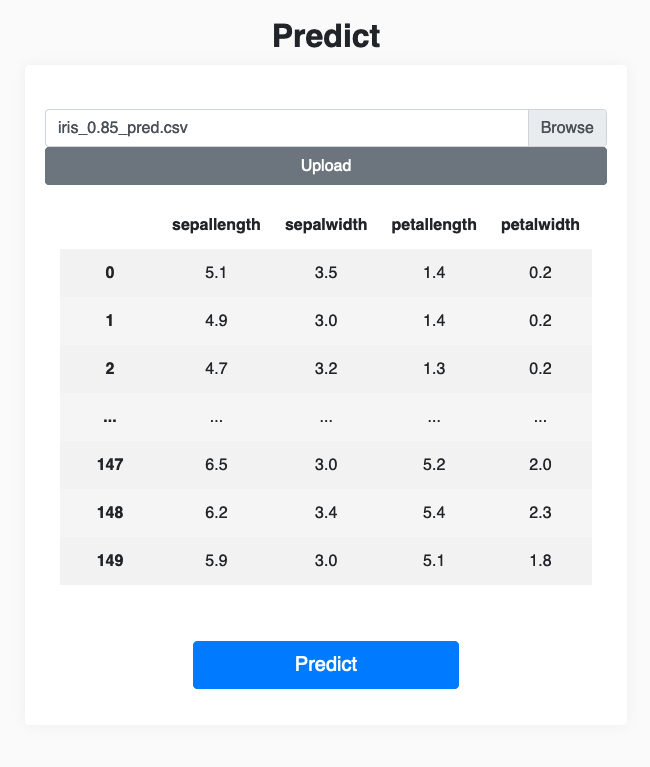
\includegraphics[scale=0.4]{../img/anexos/manual-usuario/UBUMLaaS/pre-predict}
\caption{Vista de antes de predecir.}\label{fig:pre-predict}
\end{figure}

Y posterior a la predicción se mostrarán los resultados tal y como cabría esperar, en la Figura~\ref{fig:post-predict} se muestra el ejemplo, en caso de considerar que la predicción es correcta, se mostrará en verde, en este caso todas son rojas puesto que no se garantiza su corrección.

\begin{figure}
\centering
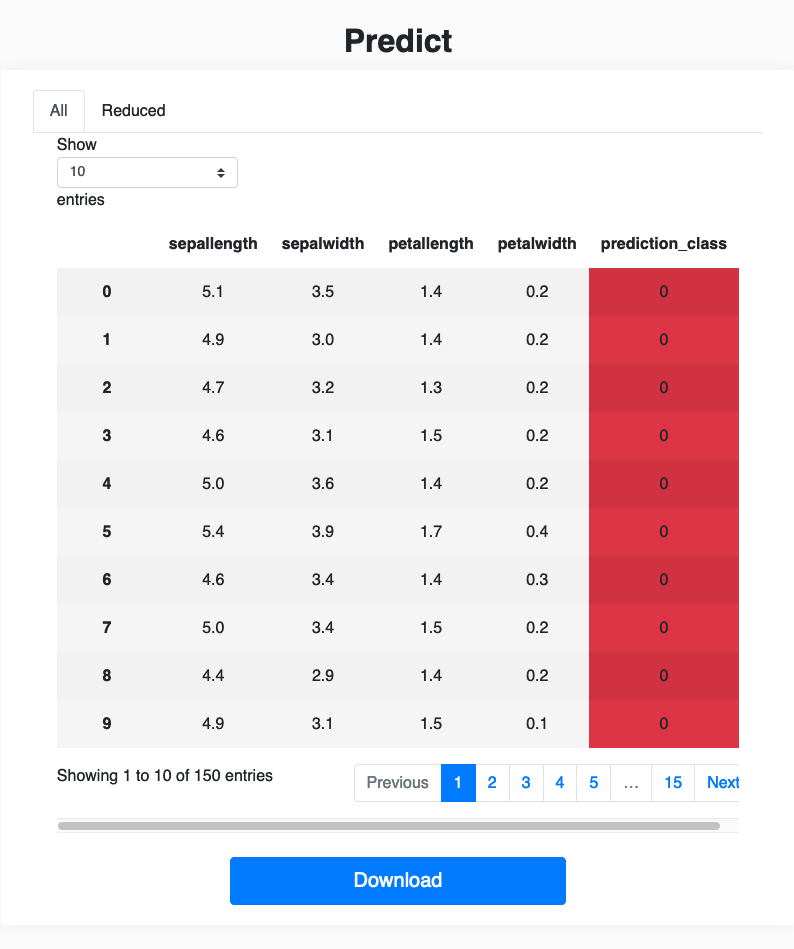
\includegraphics[scale=0.4]{../img/anexos/manual-usuario/UBUMLaaS/post-predict}
\caption{Vista de después de predecir.}\label{fig:post-predict}
\end{figure}

\FloatBarrier
\subsubsection{Estadísticas de uso}
Si se desean visualizar las estadísticas personales de uso de la aplicación, se debe acudir al perfil del usuario, el cuál es compartido con la lista de experimentos, desde la pantalla principal, Figura~\ref{fig:index-login}, (o desde cualquier otra) se deberá pulsar en la parte superior derecha sobre el botón \textit{Launched Experiments}, y se redirigirá al perfil. 

En el perfil, Figura~\ref{fig:profile}, se pulsará sobre el botón verde debajo de la foto de perfil del usuario en el lado izquierdo, el botón muestra una cadena de texto en la que se indica \textit{Statistics}. Seguidamente se abrirá una nueva \texttt{card} a la derecha, encima de todo lo que aparece, con las estadísticas del usuario. Para cerrar la vista basta con hacer \textit{click} de nuevo sobre el botón verde o sobre la cabecera de la \texttt{cart}. 

En la Figura~\ref{fig:user-stats} se muestra un ejemplo de las estadísticas de un usuario, las comentamos al detalle a continuación:
\begin{itemize}
\item Las cartas superiores son dos contadores, indican los experimentos \textbf{existentes} en la base de datos de la aplicación con identificador de usuario igual al usuario en cuestión. Y la segunda indica el número de conjunto de datos que el usuario posee en total, incluyendo los añadidos por defecto.
\item El gráfico titulado \textit{Experiments performed in the last 7 days}, tal y como la traducción referencia, muestra un gráfico con el número de experimentos que se han ejecutado por parte del usuario en los últimos 7 días, siendo el valor más a la derecha el día actual.
\item El gráfico de tipo \textit{pie} muestra el número de experimentos de cada tipo que el usuario ha ejecutado.
\item El gráfico de barras permite conocer el tiempo en total que los experimentos de un usuario han estado en ejecución en el sistema, estando agrupados por tipos de algoritmos. Se puede cambiar la escala de tiempo para una mayor comodidad de interpretación.
\end{itemize}

\imagenFlotante{../img/anexos/manual-usuario/UBUMLaaS/user-stats}{Estadísticas de usuario.}{user-stats}

\FloatBarrier
\subsubsection{Modificación de datos del usuario y actualizar contraseña}
Todo usuario puede modificar sus datos personales, así como añadir una serie de datos que no son obligatorios. Para modificar los datos se realizará desde el perfil del usuario, haciendo \textit{click} en el botón amarillo en la parte inferior izquierda, con la cadena de caracteres \textit{Edit profile}.

En este momento se lanzará un modal el cual posee dos partes diferencias, modificación de datos personales, y en la parte inferior modificación de la contraseña.

Cuando se decida qué se quiere modificar, se deberá hacer \textit{click} en el \textit{checkbox} que se encuentra en la parte superior de cada formulario, lo cual habilitará la edición del mismo. Los formularios se encuentran en las Figuras~\ref{fig:edit-profile-data}~y~\ref{fig:edit-profile-passwd}, respectivamente. 

\begin{figure}
\centering
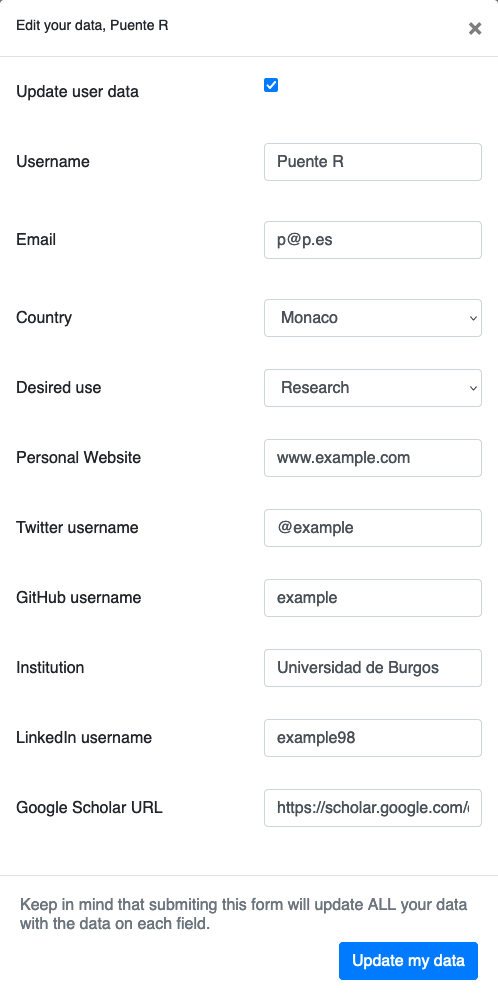
\includegraphics[scale=0.5]{../img/anexos/manual-usuario/UBUMLaaS/edit-profile-data}
\caption{Formulario de edición de los datos de un usuario.}\label{fig:edit-profile-data}
\end{figure}

\begin{figure}
\centering
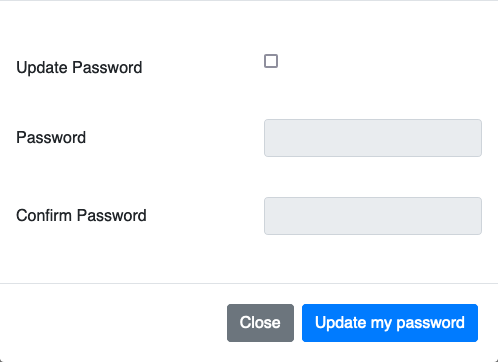
\includegraphics[scale=0.5]{../img/anexos/manual-usuario/UBUMLaaS/edit-profile-passwd}
\caption{Formulario para cambiar la contraseña de un usuario.}\label{fig:edit-profile-passwd}
\end{figure}

\FloatBarrier
\subsection{Manual del administrador}
A continuación se detallan todas las funcionalidades añadidas que posee un administrador. Un administrador es un usuario en su base, por lo tanto, todas las funcionalidades descritas en la sección anterior también hacen referencia al administrador.

\subsubsection{\texttt{NavBar} de administración}
Tal y como se aprecia en la Figura~\ref{fig:index-admin}, el administrador posee una barra de navegación lateral en toda la aplicación, permitiendo acceder a esas funcionalidades en cualquier momento desde cualquier lugar. A su vez, en la parte superior derecha posee un acceso directo a la parte de administración, el botón \textit{Administration}.

En caso de querer ocultar la barra lateral de administración, ya que no se va utilizar en ese momento, en la parte superior izquierda aparece una \texttt{X}, haciendo \textit{click} en ella se ocultará la barra lateral.

\imagenFlotante{../img/anexos/manual-usuario/UBUMLaaS/index-admin}{Vista principal de administrador.}{index-admin}

En las siguientes secciones se comentarán cada una de las opciones disponibles para los administradores.

\subsubsection{Analytics Dashboard}
Accediendo a través del botón \textit{Dashboard} en el menú lateral, se accede a la vista de analíticas del sistema, en la que aparecen tanto estadísticas de los últimos 7 días, como globales del sistema, se puede apreciar en la Figura~\ref{fig:dashboard}.

\imagenFlotante{../img/anexos/manual-usuario/UBUMLaaS/dashboard}{Vista de \textit{Analytics Dashboard}.}{dashboard}

Se dispone de la siguiente información:
\begin{itemize}
\item Cartas superiores
\begin{itemize}
	\item Número total de experimentos (los modelos) que se encuentran almacenados en el sistema.
	\item Número total de conjuntos de datos distintos almacenados en el sistema.
	\item Número de usuarios registrados en el sistema.
	\item Número total del países de los cuáles los usuarios han dicho ser.
\end{itemize}
\item \textit{Experiments performed in the last 7 days}. Igual que para el usuario, pero con las estadísticas de todos los usuarios. 
\item \textit{Algorithm Type Usage Distribution}. Estadísticas globales del número de experimentos de cada tipo que se han ejecutado.
\item \textit{Algorithm Type Time Used}. Distribución del tiempo de uso (ejecución) de los diferentes tipos de algoritmos.
\item \textit{Desired Use}. Estadísticas del uso que los usuarios han indicado que le van a dar primordialmente a la aplicación.
\item \textit{Country Distribution}. Representación de la ubicación geográfica de los usuarios. Siendo representado cada país por un único punto.
\item \textit{Latests Experiments}. Últimos 10 experimentos lanzados, pueden estar \textit{In Progress}, o terminados, ya sea \textit{Finalized} o bien \textit{Error}. Mostrando la información mínima necesaria así como el usuario dueño del experimento.
\item \textit{All Time Datasets Run}. Comparativa del tiempo de ejecución de algunos conjuntos de datos en comparación con el número de veces que han sido ejecutados. Se puede modificar la escala de tiempo.
\end{itemize}

\subsubsection{Users}
Se accede a la página de administración de usuarios a través del botón \textit{Users} en la barra lateral. En este panel se pueden crear, (des)activar, dar/quitar privilegios de administración, o eliminar un usuario.

Tal y como se puede ver en la Figura~\ref{fig:users-admin}, se soporta la búsqueda por cualquiera de los campos que se visualizan, permitiendo encontrar a aquellos usuarios que interese en <<un \textit{click}>>. 

\imagenFlotante{../img/anexos/manual-usuario/UBUMLaaS/users-admin}{Vista de administración de usuarios.}{users-admin}

Un usuario no puede quitarse a sí mismo privilegios de administrador, ni deactivarse la cuenta, o eliminarla, teniendo que ser otro administrador el que lo haga; de esta manera el sistema siempre tendrá como mínimo un administrador.

A su vez se soporta crear un usuario haciendo \textit{click} en el botón verde \textit{New user}. Desplegándose un formulario y se deberán de rellenar los campos de correo electrónico, nombre de usuario, país y uso que se va a hacer; las restricciones de los campos existentes deben de seguir cumpliéndose. Al usuario se le generará una contraseña y al correo electrónico llega un correo, valga la redundancia, de activación de la cuenta, pero deberá de re-establecer la contraseña como si la hubiera olvidado antes de poder iniciar sesión por primera vez.

\subsubsection{Live System Monitor}
A la monitorización del sistema en tiempo real se accede a través del botón \textit{Live System Monitor} en la barra lateral. Cuando se hace \textit{click} se redirecciona a una vista similar a la que aparece en la Figura~\ref{fig:live-monitor}. En la parte superior derecha de la página a la que se llega hay un botón para activar si se quiere que la página se auto-recargue cada 60 segundos, desde el momento en el que se hace \textit{click}.

\imagenFlotante{../img/anexos/manual-usuario/UBUMLaaS/live-monitor}{Vista de \textit{Live System Monitor}.}{live-monitor}

\textbf{NOTA.} Es importante tener en cuenta que esta pantalla se ha diseñado para monitores de más de 23 pulgadas, por lo que su visualización en monitores de menor tamaño puede no ser óptima o encontrar ciertos solapamientos. En la Figura~\ref{fig:live-monitor} se aprecia la disposición correcta de todos los componentes.

La información que se muestra es la siguiente (todas las unidades que se muestran son calculadas dinámicamente, seleccionando la mayor disponible):
\begin{itemize}
\item Las cartas superiores muestran, de izquierda a derecha:
\begin{itemize}
	\item \textit{CPU Load}. La carga de la CPU porcentualmente.
	\item \textit{CPU Cores}. El número total de núcleos del sistema.
	\item \textit{Memory Load}. El uso total de la memoria en forma de gráfico.
	\item \textit{Used Memory}. El valor total de memoria en uso en el sistema.
	\item \textit{Storage in use}. Almacenamiento total del sistema en vista de gráfico.
	\item \textit{Storaged Used}. El valor total de almacenamiento en uso.
\end{itemize}
\item \textit{System Load 1/5/15}. Cada gráfico representa la carga media del sistema en los últimos 1, 5 y 15 minutos, respectivamente.
\item \textit{I/O Usage}. Interrupciones de tipo \textit{Input}/\textit{Output} de la CPU y del disco.
\item \textit{Network Usage}. Tamaño total de información transmitida y recibida en el periodo de tiempo.
\item Las cartas inferiores muestran, de izquierda a derecha:
\begin{itemize}
	\item \textit{Uptime}. Tiempo total desde que el sistema se inició. Formato: días:horas:minutos:segundos.
	\item \textit{IP Address}. Dirección IP del equipo/servidor donde se encuentra la plataforma desplegada.
	\item \textit{IP Public Address}. Dirección IP pública del sistema.
	\item \textit{IP Mask CIDR}. Máscara de subred en formato CIDR.
	\item \textit{Total Processes}. Número total de procesos que existen en el sistema en ejecución.
	\item \textit{Total Threads}. Número total de hilos en el sistema.
\end{itemize}
\end{itemize}

%%%%%%%%%%%%%%%%%%%%%%%%%%%%%%%%%%%%%%%%%%%%%%%%%%%%%%%%%%%%%%%%%%%%%%
\FloatBarrier
\clearpage
\section{IS-SSL}
A continuación se presenta el manual de usuario de las bibliotecas de algoritmos desarrolladas. Permitiendo a cualquier usuario comprender \texttt{IS-SSL} y poder hacer uso de las mismas.
\subsection{Requisitos de usuarios}
Los requisitos mínimos para poder hacer uso de \texttt{IS-SSL} son:
\begin{itemize}
\item Tener instalado Python 3.7+.
\item Tener instalado y configurado \texttt{PIP} o \texttt{Conda}.
\item Disponer de un editor de textos.
\item Tener instaladas las bibliotecas necesarias para su correcto funcionamiento.
\end{itemize}

\subsection{Instalación}

Por comodidad para el usuario, \texttt{IS-SSL} se ha dividido en dos bibliotecas, una formada por los algoritmos de selección de instancias, y una segunda por aquellos algoritmos de aprendizaje semi-supervisado.

El proceso de instalación de cualquiera de las dos bibliotecas es muy sencillo, siendo integrable en cualquier fichero de requerimientos, ya sea para \texttt{PIP} o \texttt{Conda}.

Las dos bibliotecas se encuentran publicadas en PyPI\footnote{\textit{Python Package Index} es un repositorio de \textit{software} para el lenguaje de programación de Python.} desde su versión 1.0, la cual fue una primea versión alpha estable con los primeros algoritmos publicados. 
La versión 3.3 es la versión estable (la final) que se ha publicado.

\imagenFlotante{../img/anexos/manual-usuario/PyPI-IS}{Vista de la biblioteca de algoritmos de selección de instancias en PyPI.}{PyPI-IS}
\imagenFlotante{../img/anexos/manual-usuario/PyPI-SSL}{Vista de la biblioteca de algoritmos de aprendizaje semi-supervisado en PyPI.}{PyPI-SSL}

Para realizar la instalación se deben seguir los siguientes pasos para cualquier LIB, LIB $\in \lbrace$ IS-DNX, SSL-DNX$\rbrace$.

\begin{enumerate}
\item Acceder a PyPi, desde~\cite{PyPI}.
\item Introducir en el campo de búsqueda <<LIB>>.
\item Seleccionar la biblioteca correspondiente de entre la lista mostrada.
\item Copiar el comando de instalación.
\item Abrir una terminal con soporte a Python y \texttt{PIP}.
\item Introducir el comando copiado.
\item En caso de que se nos pregunte si se quiere proceder con la descarga, indicar que sí con una S en caso de que esté en español, o con Y en el caso inglés/internacional.
\item Cuando finaliza la instalación, la biblioteca se encontrará lista para su uso.
\end{enumerate}

\imagenFlotante{../img/anexos/manual-usuario/PIP-IS}{Instalación de la biblioteca de selección de instancias.}{PIP-IS}
\imagenFlotante{../img/anexos/manual-usuario/PIP-SSL}{Instalación de la biblioteca de semi-supervisado.}{PIP-SSL}


\subsection{Manual del usuario}

A continuación se documentan las funcionalidades de las bibliotecas, desde su importación, a uso y especificación de los diferentes parámetros de entrada y salida esperados. A modo de resumen se puede destacar que todos los algoritmos siguen la misma estructura interna luego el aprendizaje y familizarización es relativamente rápido.

\subsubsection{Biblioteca de algoritmos de selección de instancias}
\textbf{Importar}\\
Para poder trabajar con los algoritmos de selección de instancias se deben de importar en el fichero en el que se quieran utilizar. Para ello se importan como cualquier otro paquete de Python, supongamos que queremos utilizar el algoritmo ENN, lo importaremos de la siguiente manera:

\texttt{from InstanceSelectionDNX import ENN} 

De esta forma podemos sustituir ENN por el algoritmo que deseemos de entre los disponibles y tenerlo a nuestra disposición para su uso.

Todos los algoritmos están codificados como \texttt{class} por lo tanto se debe de instanciar antes de poder hacer uso del mismo. 

\textbf{Uso}\\
Como se ha comentado al comienzo, todos los algoritmos poseen la misma estructura. Todos ellos poseen el método \texttt{filter} de tal manera que una vez se haya instanciado se podrá llamar al método y se obtendrá como resultado el conjunto de datos reducido.

Todos los algoritmos en su instanciación reciben aquellos parámetros que son necesarios para la configuración y su uso posterior, mientras que cuando se realiza el filtrado únicamente reciben el conjunto de datos dividido, por un lado los atributos y por otro lado la clase.

Tanto las entradas como las salidas deben ser objetos de tipo \texttt{DataFrame} de \texttt{Pandas}.

\begin{lstlisting}[language=python, caption={Ejemplo de uso de ENN}]]
from InstanceSelectionDNX import ENN
import pandas as pd

data = pd.DataFrame([[1, 2, 3, 4],
        [4, 3, 2, 1],
        [1, 2, 4, 3],
        [2, 1, 3, 4]])
target = pd.DataFrame([0, 0, 1, 1])

model = ENN(nearest_neighbors=3, power_parameter=2)

data_red, label_red = model.filter(data, target)
\end{lstlisting}

\subsubsection{Biblioteca de algoritmos de aprendizaje semi-supervisado}
\textbf{Importar}\\
De manera análoga a la otra biblioteca, importaremos el paquete y seleccionaremos cuál es el algoritmo que se desea utilizar, por ejemplo:

\texttt{from SemiSupervisedLearningDNX import TriTraining}\\
Pudiendo sustituir TriTraining por el algoritmo deseado.\\
Todos los algoritmos están codificados como \texttt{class} por lo tanto se debe de instanciar antes de poder hacer uso del mismo. 

\textbf{Uso}\\
Los algoritmos siguen la misma estructura interna que los propios de \texttt{Scikit-Learn}, por lo que una vez instanciados (con sus respectivos parámetros de configuración) bastará con llamar al método \texttt{fit} de cada uno de ellos, así como para predecir al método correspondiente, denominado \texttt{predict}.

\begin{itemize}
\item \textbf{\texttt{fit}:} recibe como argumentos dos parámetros, las instancias y las etiquetas o clases, siendo -1 aquellas que se desconozcan y se quieran utilizar para entrenar el algoritmo.
\item \textbf{\texttt{predict}:} recibe únicamente las instancias que se quieren etiquetar. Devuelve estas instancias etiquetadas.
\end{itemize}

\begin{lstlisting}[language=Python, caption={Ejemplo de uso de IS-SSL}, label={lst:ejemplossl}]
from SemiSupervisedLearningDNX import TriTraining
from sklearn.naive_bayes import GaussianNB
from sklearn.neighbors import KNeighborsClassifier
from sklearn.datasets import load_iris
	
model = TriTraining(
	random_state = 42,
	c1 = GaussianNB, c1_params = None,
	c2 = KNeighborsClassifier, c2_params = {n_neighbors: 2}
)
	
iris = load_iris()
X = iris['data']
y = iris['target']

X = pd.DataFrame(X), y = pd.DataFrame(y)
	
val = [True if i % 2 == 0 else False for i in range(len(y))]
y.loc[val] = -1

X, X_test, y, y_test = train_test_split(X.to_numpy(), y.to_numpy())

X = pd.DataFrame(X), y = pd.DataFrame(y)

model.fit(X, y)
y_pred = model.predict(X_test)
	
\end{lstlisting}
\subsubsection{Ejemplo de uso combinado de ambas bibliotecas}
\begin{lstlisting}[language=Python, caption={Ejemplo de uso de IS-SSL}, label={lst:ejemplo}]
from SemiSupervisedLearningDNX import TriTraining
from InstanceSelectionDNX import ENN
from sklearn.naive_bayes import GaussianNB
from sklearn.neighbors import KNeighborsClassifier
from sklearn.tree import DecisionTreeClassifier
from sklearn.datasets import load_iris
	
if __name__ == "__main__":
	model = TriTraining(
		random_state = 42,
		c1 = GaussianNB, c1_params = None,
		c2 = KNeighborsClassifier, c2_params = {n_neighbors: 2},
		c3 = DecisionTreeClassifier, c3_params = None	
	)
	filter_model = ENN(nearest_neighbors = 5, power_parameter = 2)
	
	iris = load_iris()
	X = iris['data']
	y = iris['target']

	X = pd.DataFrame(X)
	y = pd.DataFrame(y)
	X, y = filter_model.filter(X, y)

	val = [True if i % 2 == 0 else False for i in range(len(y))]
	y[val] = -1

	X, X_test, y, y_test = train_test_split(X.to_numpy(), y.to_numpy())

	X = pd.DataFrame(X)
	y = pd.DataFrame(y)

	model.fit(X, y)
	y_pred = model.predict(X_test)
	print(accuracy_score(y_true=y_test, y_pred=y_pred))
	
\end{lstlisting}


\bibliographystyle{plain}
\bibliography{bibliografiaAnexos}

\end{document}
